% !TeX program = xelatex
\documentclass[10pt, a4paper]{article}

\usepackage{amsmath, amssymb, amsthm, mathtools}
\usepackage{geometry}
\usepackage{fancyhdr}
\usepackage{enumitem}
\usepackage{titlesec}
\usepackage{tocloft}
\usepackage[x11names]{xcolor}
\usepackage{graphicx}
\usepackage{float}
\usepackage{booktabs}
\usepackage{multirow}
\usepackage{caption}
\usepackage{subcaption}
\usepackage{tikz}
\usepackage{microtype}
\usepackage{listings}
\usepackage[most]{tcolorbox}
\tcbuselibrary{skins, breakable}
\usepackage[backend=biber, citestyle=numeric-comp, bibstyle=numeric]{biblatex}
\usepackage{hyperref}
\usepackage[capitalise, noabbrev]{cleveref}

\usetikzlibrary{arrows.meta, calc, decorations.pathmorphing, positioning}

% --- Palette: Navy + Amber Gold ---
\definecolor{primary}{RGB}{28, 55, 90}
\definecolor{accent}{RGB}{176, 128, 52}
\definecolor{accentlight}{RGB}{232, 214, 178}
\definecolor{problembg}{RGB}{250, 248, 243}
\definecolor{problemframe}{RGB}{210, 220, 232}
\definecolor{textmuted}{RGB}{95, 105, 118}
\definecolor{coverbg}{RGB}{252, 249, 238}
\definecolor{progcolor}{RGB}{52, 105, 88}

% --- Page Geometry & Header/Footer ---
\geometry{left=2.4cm, right=2.4cm, top=2.6cm, bottom=2.6cm}
\setlength{\headheight}{18pt}
\setlength{\parindent}{1.5em}
\setlength{\parskip}{0.38em}
\linespread{1.15}
\emergencystretch=2em
\setlist{nosep, leftmargin=1.8em}

\pagestyle{fancy}
\fancyhf{}
\fancyhead[L]{\small\color{primary}\textsf{ADS Project 1: Compare Search Trees}}
\fancyhead[R]{\small\color{textmuted}\textsf{Fall--Winter 2026}}
\fancyfoot[C]{\small\color{textmuted}\thepage}
\renewcommand{\headrulewidth}{0.5pt}
\renewcommand{\headrule}{%
  {\color{accent!55}\hrule width\headwidth height 0.5pt}%
}

% --- Section & Subsection Headings ---
\titleformat{\section}
  {\color{primary}\centering\Large\bfseries}
  {\color{accent}Chapter~\thesection.}{0.6em}{}
  [\vspace{0.3em}{\color{accent!70}\titlerule[1.5pt]}]

\titleformat{name=\section,numberless}
  {\color{primary}\centering\Large\bfseries}
  {}{0pt}{}
  [\vspace{0.3em}{\color{accent!70}\titlerule[1.5pt]}]

\titleformat{\subsection}
  {\color{primary!88!black}\large\bfseries}
  {\color{accent}\thesubsection}{0.6em}{}
  [\vspace{0.15em}{\color{accent!45}\titlerule[0.8pt]}]

\titleformat{\subsubsection}
  {\color{primary!85!black}\normalsize\bfseries}
  {\color{accent}\thesubsubsection}{0.5em}{}

\titlespacing*{\section}{0pt}{0.6em}{1.0em}
\titlespacing*{\subsection}{0pt}{1.0em}{0.6em}
\titlespacing*{\subsubsection}{0pt}{0.8em}{0.4em}

% --- TOC Styling ---
\renewcommand{\cftsecfont}{\bfseries\color{primary}}
\renewcommand{\cftsecpagefont}{\bfseries\color{primary}}
\renewcommand{\cftsubsecfont}{\color{black!85}}
\renewcommand{\cftsubsubsecfont}{\small\color{textmuted}}
\setlength{\cftbeforesecskip}{0.55em}

% --- Styled Boxes ---
\newtcolorbox{insightbox}[1]{
    enhanced,
    breakable,
    colback=progcolor!5.5,
    colframe=progcolor!28,
    boxrule=0.7pt,
    arc=4pt,
    borderline west={3.5pt}{0pt}{progcolor},
    left=13pt,
    right=13pt,
    top=9pt,
    bottom=11pt,
    before skip=10pt plus 2pt,
    after skip=12pt plus 2pt,
    title={\sffamily #1},
    fonttitle=\bfseries,
    coltitle=white,
    colbacktitle=progcolor,
    attach boxed title to top left={yshift=-2mm, xshift=8mm},
    boxed title style={
        arc=2.5pt,
        boxrule=0pt,
        top=2pt,
        bottom=2pt,
        left=7pt,
        right=7pt,
    },
}

% --- Code Listings & Captions ---
\newcommand{\code}[1]{\texttt{\color{primary!90!black}#1}}
\newcommand{\bfactor}[1]{\ensuremath{\mathrm{BF}(#1)}}
\newcommand{\kw}[1]{\textbf{\color{primary}#1}}
\newcommand{\id}[1]{\ensuremath{\mathrm{#1}}}
\captionsetup{labelfont={bf,color=primary}, skip=4pt}
\BeforeBeginEnvironment{tabular}{\small}

\lstset{
    language=C,
    basicstyle=\ttfamily\scriptsize,
    keywordstyle=\color{primary}\bfseries,
    commentstyle=\color{progcolor}\itshape,
    stringstyle=\color{accent},
    breaklines=true,
    numbers=left,
    numberstyle=\tiny\color{textmuted},
    frame=single,
    rulecolor=\color{problemframe},
    backgroundcolor=\color{problembg},
    captionpos=b,
    tabsize=4,
    columns=fullflexible,
    showstringspaces=false
}

\tikzset{
    avlnode/.style={circle, draw=primary, very thick, fill=primary!8, minimum size=7.5mm, font=\small\bfseries, text=primary},
    avledge/.style={-{Stealth[length=2mm]}, thick, primary},
    rbblack/.style={circle, draw=primary!95!black, very thick, fill=primary!90!black, minimum size=5.2mm, inner sep=0pt, font=\scriptsize\bfseries, text=white},
    rbred/.style={circle, draw=Red3, very thick, fill=Red3!14, minimum size=5.2mm, inner sep=0pt, font=\scriptsize\bfseries, text=Red3!90!black},
    rbany/.style={circle, draw=accent!90!black, very thick, fill=accent!22, minimum size=5.2mm, inner sep=0pt, font=\scriptsize\bfseries, text=primary},
    rbdouble/.style={circle, draw=primary!95!black, double=white, double distance=1.0pt, very thick, fill=primary!90!black, minimum size=5.2mm, inner sep=0pt, font=\scriptsize\bfseries, text=white}
}

\hypersetup{
    colorlinks=true,
    linkcolor=primary,
    citecolor=progcolor,
    urlcolor=accent,
    linktoc=all
}

\graphicspath{{../src/visualizations/}{image/}{figure/}{fig/}{img/}}
\addbibresource[location=local]{reference.bib}

\begin{document}

% ============================================================
%  PAGE 1: DEDICATED COVER + ABSTRACT PAGE
% ============================================================
\begin{titlepage}
\begin{tikzpicture}[remember picture, overlay]
    \fill[coverbg] (current page.south west) rectangle (current page.north east);
    \draw[accent!40, line width=0.7pt]
        ([xshift=1.5cm, yshift=-1.5cm]current page.north west) --
        ([xshift=1.5cm, yshift=1.5cm]current page.south west);
    \draw[accent!40, line width=0.7pt]
        ([xshift=-1.5cm, yshift=-1.5cm]current page.north east) --
        ([xshift=-1.5cm, yshift=1.5cm]current page.south east);
    \foreach \r in {2.0, 2.45, 2.9} {
        \draw[primary!14, line width=0.5pt]
            ([xshift=-1.35cm, yshift=1.35cm]current page.south east) circle (\r cm);
        \draw[primary!14, line width=0.5pt]
            ([xshift=1.35cm, yshift=-1.35cm]current page.north west) circle (\r cm);
    }
\end{tikzpicture}

\vspace*{0.8cm}
\begin{center}
    {\large\color{accent}\textsf{\textbf{Advanced Data Structures and Algorithm Analysis}}}\\[0.25cm]
    {\normalsize\color{textmuted}\textsf{Laboratory Project Report $\cdot$ Project 1}}\\[0.6cm]

    {\color{primary}\rule{0.58\textwidth}{1.4pt}}\\[0.55cm]
    {\fontsize{23}{30}\selectfont\bfseries\color{primary} Performance Comparison and}\\[0.2cm]
    {\fontsize{23}{30}\selectfont\bfseries\color{primary} Analysis of Search Trees}\\[0.45cm]
    {\color{accent}\rule{0.24\textwidth}{1.0pt}}\\[0.85cm]

    {\Large\bfseries\color{primary} Student A \hspace{2.8em} Student B}\\[0.35cm]
    {\normalsize\color{textmuted}
        Zhejiang University \\[0.15cm]
        Date: 2026-10-19
    }
\end{center}

\vspace{0.8cm}
\begin{center}
    {\large\bfseries\color{primary} Abstract}
\end{center}
\vspace{-0.2em}
\begin{quote}
\small\noindent
Search trees serve as fundamental building blocks for dynamic ordered dictionaries in both in-memory runtime libraries and external-storage indexing engines. In this project, we implement five representative search tree structures in C: the \textbf{unbalanced Binary Search Tree}, \textbf{AVL Tree}, \textbf{Splay Tree}, \textbf{Red-Black Tree}, and order-$4$ \textbf{$\text{B}^+$ Tree}. To evaluate their \textbf{asymptotic complexity} and structural resilience through \textbf{empirical benchmarking}, we test all five trees over datasets of $N$ distinct integers ranging from $1{,}000$ to $50{,}000$ under three canonical workloads: \textbf{increasing-order insertion and increasing-order deletion}, \textbf{increasing-order insertion and reverse-order deletion}, and \textbf{random-order insertion and random-order deletion}. At $N=50{,}000$, empirical measurements confirm that while an unbalanced BST achieves the lowest constant-factor overhead on randomized inputs with $5.52\,\text{ms}$ insertion and $5.36\,\text{ms}$ deletion, it suffers catastrophic $\Theta(N^2)$ degeneration on monotone sequences, taking $1.89\,\text{s}$ for insertion and $1.78\,\text{s}$ for reverse deletion. Conversely, Splay Trees exploit sequential spatial locality to achieve $\Theta(N)$ total time of $0.78\,\text{ms}$ for sorted insertions, Red-Black Trees offer the most consistent all-around performance across adversarial and random workloads through bounded rotation counts, AVL Trees trade higher rotation frequency for stricter height bounds, and $\text{B}^+$ Trees incur higher CPU array-shifting overhead per update.

\vspace{0.55em}\noindent
{\color{primary}\textbf{Keywords:}} Binary search tree; AVL tree; splay tree; red-black tree; $\text{B}^+$ tree; empirical benchmarking; asymptotic complexity.
\end{quote}

\vfill
\begin{center}
    {\color{accent!80}\rule{0.14\textwidth}{0.8pt}}\\[0.25cm]
    {\normalsize\bfseries\color{primary} Fall--Winter 2026}
\end{center}
\end{titlepage}

% ============================================================
%  PAGE 2: DEDICATED TABLE OF CONTENTS PAGE
% ============================================================
\pagenumbering{roman}
\thispagestyle{plain}
\vspace*{0.3cm}
\tableofcontents
\clearpage

% ============================================================
%  CHAPTER 1: INTRODUCTION
% ============================================================
\pagenumbering{arabic}
\section{Introduction}

\subsection{Problem Description}
Maintaining a dynamic collection of ordered keys under frequent insertions, deletions, and lookups is a core problem in computer science. Although an ordinary Binary Search Tree supports these dictionary operations in $O(\log N)$ time on average when keys arrive in random permutations~\cite{weiss1996}, it offers no worst-case structural guarantee. Under adversarial or naturally ordered arrival streams, an ordinary BST degenerates into a singly linked chain of height $N-1$, degrading individual updates to $\Theta(N)$ time and a sequence of $N$ operations to $\Theta(N^2)$ time.

To overcome tree degeneration without sacrificing ordered traversal semantics, four major families of self-balancing and self-adjusting search trees are covered in the ADS course lectures~\cite{ads_slides2026}:
\begin{itemize}
  \item \textbf{\color{primary}AVL Trees} enforce a strict local height-balance invariant $|\bfactor{v}| \le 1$ at every node, guaranteeing worst-case $O(\log N)$ height via single and double rotations~\cite{ads_slides2026,weiss1996}.
  \item \textbf{\color{primary}Red-Black Trees} relax the height constraint into a two-color path invariant, bounding tree height by $2\log_2(N+1)$ while restricting structural fixes to at most $O(1)$ rotations per update~\cite{ads_slides2026,cormen2022}.
  \item \textbf{\color{primary}Splay Trees} eliminate explicit balance metadata altogether, moving every accessed node to the root via two-step \emph{zig-zig} and \emph{zig-zag} rotations to guarantee $O(\log N)$ amortized cost per operation~\cite{ads_slides2026,weiss1996}.
  \item \textbf{\color{primary}$\text{B}^+$ Trees} generalize binary trees into multi-way search structures where all keys reside in linked leaf nodes and internal nodes act as routing separators, optimizing node fan-out through node splitting and merging~\cite{ads_slides2026}.
\end{itemize}

\subsection{Purpose of This Report}
The objective of this project is to implement all five search trees from scratch in C, verify their structural invariants, and systematically analyze and compare the performances of sequences of insertions and deletions across $N \in [10^3, 5\times 10^4]$ distinct integers in three canonical ways:
\begin{enumerate}[label=\textbf{\color{primary}\arabic*.}]
  \item \textbf{Ordered Insertion \& Same-Order Deletion:} Insert $N$ integers in increasing order $0, 1, \dots, N-1$ and delete them in the same increasing order;
  \item \textbf{Ordered Insertion \& Reverse-Order Deletion:} Insert $N$ integers in increasing order $0, 1, \dots, N-1$ and delete them in the reverse decreasing order $N-1, N-2, \dots, 0$;
  \item \textbf{Random Insertion \& Random Deletion:} Insert $N$ integers in a uniform random order and delete them in an independent uniform random order.
\end{enumerate}
By combining theoretical complexity proofs with detailed empirical runtime measurements, this report clarifies the practical trade-offs between height balance, color balance, self-adjustment, and multi-way branching.

\clearpage

% ============================================================
%  CHAPTER 2: DATA STRUCTURE / ALGORITHM SPECIFICATION
% ============================================================
\section{Data Structure and Algorithm Specification}

\subsection{Overview of Node Specifications}
\Cref{tab:structures} summarizes the structural metadata, invariants, and memory layouts of the five implemented search trees.

\begin{table}[H]
\centering
\caption{Comparison of structural representations and invariants across the five search trees.}
\label{tab:structures}
\begin{tabular}{@{}lp{0.33\linewidth}p{0.43\linewidth}@{}}
\toprule
\textbf{\color{primary}Structure} & \textbf{\color{primary}Node Fields} & \textbf{\color{primary}Balancing Invariant} \\
\midrule
Unbalanced BST & \code{val}, \code{Left}, \code{Right} & None; tree shape depends entirely on insertion and deletion history. \\
AVL Tree & \code{val}, \code{height}, \code{BF}, \code{Left}, \code{Right} & Height difference $|\bfactor{v}| = |h(v.\text{Left}) - h(v.\text{Right})| \le 1$ for every node $v$. \\
Splay Tree & \code{key}, \code{left}, \code{right} & No stored balance metadata; newly accessed, inserted, or split nodes are splayed to the root. \\
Red-Black Tree & \code{key}, \code{color}, \code{left}, \code{right}, \code{parent} & Root is black; red nodes have black children; every root-to-\code{NULL} path contains the same number of black nodes. \\
Order-$4$ $\text{B}^+$ Tree & \code{isLeaf}, \code{numKeys}, \code{keys[]}, \code{children[]}, \code{parent}, \code{next} & Internal nodes have $2$ to $4$ children and $1$ to $3$ separator keys; non-root leaves hold $2$ to $3$ keys and form a singly linked list. \\
\bottomrule
\end{tabular}
\end{table}

\subsection{Unbalanced Binary Search Tree}
The standard search, insertion, and deletion rules of an unbalanced BST were already covered in \emph{Fundamentals of Data Structures}, so we omit their basic specification here.

One thing worth mentioning in \code{binaray\_search\_tree.h} is that we implement both insertion and deletion in an \textbf{iterative} manner rather than a \textbf{recursive} one. When $N=50{,}000$ sorted keys are inserted, the tree degenerates into a chain of depth $N$, causing \textbf{recursive} calls to overflow the system call stack around $N \approx 26{,}000$. Using explicit \code{parent} and \code{current} pointers in an \textbf{iterative} loop reduces auxiliary stack space to $O(1)$ and avoids stack overflow.

\subsection{AVL Tree}
In \code{AVL\_tree.h}, each node stores its subtree \code{height}, with empty trees having height $-1$ and leaves height $0$, together with the balance factor $\bfactor{v} = h(v.\id{left}) - h(v.\id{right})$. After a standard BST insertion or deletion, each ancestor $v$ along the recursion return path updates its height and restores balance when $|\bfactor{v}| = 2$ according to four cases:
\begin{itemize}
  \item \textbf{\color{primary}LL Case, $\bfactor{v} = +2$ and $\bfactor{v.\id{left}} \ge 0$:} Perform a single right rotation at $v$ to lift $v.\id{left}$ as the new subtree root, as shown in \Cref{fig:avl_rotation}.
  \item \textbf{\color{primary}RR Case, $\bfactor{v} = -2$ and $\bfactor{v.\id{right}} \le 0$:} Perform a single left rotation at $v$ to lift $v.\id{right}$ as the new subtree root.
  \item \textbf{\color{primary}LR Case, $\bfactor{v} = +2$ and $\bfactor{v.\id{left}} = -1$:} Perform a left rotation at $v.\id{left}$ followed by a right rotation at $v$.
  \item \textbf{\color{primary}RL Case, $\bfactor{v} = -2$ and $\bfactor{v.\id{right}} = +1$:} Perform a right rotation at $v.\id{right}$ followed by a left rotation at $v$.
\end{itemize}

\begin{figure}[H]
\centering
\begin{tikzpicture}[x=1cm,y=0.88cm]
  \node[avlnode] (y) at (1.5,1.8) {$y$};
  \node[avlnode] (x) at (0,0) {$x$};
  \node[avlnode] (c) at (3,0) {$C$};
  \node[avlnode] (a) at (-0.8,-1.6) {$A$};
  \node[avlnode] (b) at (0.8,-1.6) {$B$};
  \draw[avledge] (y)--(x); \draw[avledge] (y)--(c);
  \draw[avledge] (x)--(a); \draw[avledge] (x)--(b);
  \node[font=\small\bfseries\color{primary}] at (1.5,-2.35) {Before: LL imbalance, $\bfactor{y}=+2$};
  \draw[-{Stealth[length=3mm]},very thick,accent] (3.9,0.15) -- (6.5,0.15) node[midway,above=6pt,font=\small\bfseries\color{accent}]{Right-Rotate $y$};
  \node[avlnode] (xx) at (9.1,1.8) {$x$};
  \node[avlnode] (aa) at (7.4,0) {$A$};
  \node[avlnode] (yy) at (10.6,0) {$y$};
  \node[avlnode] (bb) at (9.8,-1.6) {$B$};
  \node[avlnode] (cc) at (11.4,-1.6) {$C$};
  \draw[avledge] (xx)--(aa); \draw[avledge] (xx)--(yy);
  \draw[avledge] (yy)--(bb); \draw[avledge] (yy)--(cc);
  \node[font=\small\bfseries\color{primary}] at (9.3,-2.35) {After: height balanced};
\end{tikzpicture}
\caption{AVL LL single right rotation preserving in-order key sequence $A < x < B < y < C$.}
\label{fig:avl_rotation}
\end{figure}

\begin{table}[H]
\centering
\begin{tabular}{@{}p{1.2cm}p{0.84\textwidth}@{}}
\toprule
\multicolumn{2}{@{}l}{\textbf{\color{primary}Algorithm 1:} $\id{Rebalance\text{-}AVL}(v)$} \\
\midrule
1. & Update $h(v) \gets 1 + \max(h(v.\id{left}), h(v.\id{right}))$ and $\bfactor{v} \gets h(v.\id{left}) - h(v.\id{right})$. \\
2. & \kw{if} $\bfactor{v} > 1$ \kw{then} \hfill $\triangleright$ Left-heavy subtree \\
3. & \quad \kw{if} $\bfactor{v.\id{left}} < 0$ \kw{then} $v.\id{left} \gets \id{Left\text{-}Rotate}(v.\id{left})$ \hfill $\triangleright$ Convert LR to LL \\
4. & \quad \kw{return} $\id{Right\text{-}Rotate}(v)$ \\
5. & \kw{if} $\bfactor{v} < -1$ \kw{then} \hfill $\triangleright$ Right-heavy subtree \\
6. & \quad \kw{if} $\bfactor{v.\id{right}} > 0$ \kw{then} $v.\id{right} \gets \id{Right\text{-}Rotate}(v.\id{right})$ \hfill $\triangleright$ Convert RL to RR \\
7. & \quad \kw{return} $\id{Left\text{-}Rotate}(v)$ \\
8. & \kw{return} $v$ \\
\bottomrule
\end{tabular}
\end{table}

\subsection{Splay Tree}
In \code{splay\_tree.h}, $\id{Splay}(v, k)$ moves the accessed key or the last visited node $x$ to the root via three rotation steps according to the relative positions of $x$, its parent $p$, and its grandparent $g$~\cite{ads_slides2026,weiss1996}:
\begin{itemize}
  \item \textbf{\color{primary}Zig Step:} When $p$ is the tree root, perform a single rotation at $p$ to lift $x$ directly to the root.
  \item \textbf{\color{primary}Zig-Zig Step:} When $x$ and $p$ are both left children or both right children, rotate first at the grandparent $g$ and then at the parent $p$, which halves the depth of nodes along the access path.
  \item \textbf{\color{primary}Zig-Zag Step:} When $x$ is a left child and $p$ is a right child, or vice versa, rotate first at $p$ and then at $g$, matching the double rotation of an AVL tree.
\end{itemize}
Based on $\id{Splay}(r, k)$, the insertion and deletion algorithms follow directly as shown below:

\begin{table}[H]
\centering
\begin{tabular}{@{}p{1.2cm}p{0.84\textwidth}@{}}
\toprule
\multicolumn{2}{@{}l}{\textbf{\color{primary}Algorithm 2:} $\id{Splay\text{-}Insert}(r, k)$ and $\id{Splay\text{-}Delete}(r, k)$} \\
\midrule
\textbf{Insert:} &
1. \kw{if} $r = \id{NIL}$ \kw{then return} a new single-node tree with key $k$. \\
& 2. $r \gets \id{Splay}(r, k)$; \kw{if} $r.\id{key} = k$ \kw{then return} $r$. \\
& 3. Create new root $z$ with key $k$. \kw{if} $k < r.\id{key}$ \kw{then} set $z.\id{left} \gets r.\id{left}$, $z.\id{right} \gets r$, and $r.\id{left} \gets \id{NIL}$; \kw{else} symmetrically split $r.\id{right}$. \kw{return} $z$. \\[0.35em]
\textbf{Delete:} &
1. \kw{if} $r = \id{NIL}$ \kw{then return} $\id{NIL}$. Set $r \gets \id{Splay}(r, k)$; \kw{if} $r.\id{key} \neq k$ \kw{then return} $r$. \\
& 2. \kw{if} $r.\id{left} = \id{NIL}$ \kw{then} $r' \gets r.\id{right}$; \kw{else} splay the maximum of the left subtree via $r' \gets \id{Splay}(r.\id{left}, k)$ and join $r'.\id{right} \gets r.\id{right}$. \\
& 3. Free old root $r$ and \kw{return} $r'$. \\
\bottomrule
\end{tabular}
\end{table}

\subsection{Red-Black Tree}
In \code{red\_black\_tree.h}, each node stores a color $\in \{\id{RED}, \id{BLACK}\}$ and a \code{parent} pointer. Standard BST insertion colors the new leaf $z$ $\id{RED}$; standard deletion replaces a two-child target with its in-order predecessor and removes node $y$. Violations of the red-black invariants are repaired iteratively as specified in Algorithm 3 and illustrated for all four double-black deletion cases in \Cref{fig:rb_del_cases}~\cite{ads_slides2026,cormen2022}:

\begin{table}[H]
\centering
\begin{tabular}{@{}p{1.6cm}p{0.81\textwidth}@{}}
\toprule
\multicolumn{2}{@{}l}{\textbf{\color{primary}Algorithm 3:} $\id{RB\text{-}Insert\text{-}Fixup}(z)$ and $\id{RB\text{-}Delete\text{-}Fixup}(x)$} \\
\midrule
\textbf{Insert Fix} &
Let $g = p(p(z))$ be the grandparent and $u$ be $z$'s uncle. \kw{while} $\id{color}(p(z)) = \id{RED}$ \kw{do}: \\
& $\bullet$ \textbf{Case 1, $\id{color}(u) = \id{RED}$:} Recolor $p(z), u \gets \id{BLACK}$, $g \gets \id{RED}$; advance $z \gets g$. \\
& $\bullet$ \textbf{Case 2, $u$ is $\id{BLACK}$ and $z$ is an inner grandchild:} Rotate at $p(z)$ to reduce to Case 3. \\
& $\bullet$ \textbf{Case 3, $u$ is $\id{BLACK}$ and $z$ is an outer grandchild:} Recolor $p(z) \gets \id{BLACK}$, $g \gets \id{RED}$, rotate at $g$, and \kw{break}. Finally set $\id{color}(\id{root}) \gets \id{BLACK}$. \\[0.35em]
\textbf{Delete Fix} &
Let $w$ be $x$'s sibling. \kw{while} $x \neq \id{root}$ and $\id{color}(x) = \id{BLACK}$ \kw{do}: \\
& $\bullet$ \textbf{Case 1, $\id{color}(w) = \id{RED}$:} Recolor $w \gets \id{BLACK}$, $p(x) \gets \id{RED}$, rotate at $p(x)$, and update $w$. \\
& $\bullet$ \textbf{Case 2, $w$ and both nephews are $\id{BLACK}$:} Recolor $w \gets \id{RED}$; if $p(x)$ is $\id{RED}$, color $p(x) \gets \id{BLACK}$ and \kw{break}, else advance $x \gets p(x)$. \\
& $\bullet$ \textbf{Case 3, $w$ is $\id{BLACK}$, inner nephew $\id{RED}$, outer $\id{BLACK}$:} Recolor $w$ and inner nephew, then rotate at $w$ to reduce to Case 4. \\
& $\bullet$ \textbf{Case 4, $w$ is $\id{BLACK}$ and outer nephew is $\id{RED}$:} Set $\id{color}(w) \gets \id{color}(p(x))$, $\id{color}(p(x)) \gets \id{BLACK}$, outer nephew $\gets \id{BLACK}$, rotate at $p(x)$, and \kw{break}. \\
\bottomrule
\end{tabular}
\end{table}

\vspace{-0.4em}
\begin{figure}[H]
\centering
\captionsetup[subfigure]{skip=2pt}
\begin{subfigure}[b]{0.48\textwidth}
\centering
\begin{tikzpicture}[x=0.62cm,y=0.52cm]
  \node[rbblack]  (p1) at (1.4,1.6) {$p$};
  \node[rbdouble] (x1) at (0.2,0.2) {$x$};
  \node[rbred]    (w1) at (2.6,0.2) {$w$};
  \node[rbblack]  (c1) at (1.9,-1.2) {$c$};
  \node[rbblack]  (d1) at (3.3,-1.2) {$d$};
  \draw[avledge] (p1)--(x1); \draw[avledge] (p1)--(w1);
  \draw[avledge] (w1)--(c1); \draw[avledge] (w1)--(d1);
  \draw[-{Stealth[length=2.0mm]},very thick,accent] (3.9,0.2) -- (5.5,0.2)
    node[midway,above=2pt,font=\scriptsize\bfseries\color{accent}]{Rot $p$};
  \node[rbblack]  (w2) at (7.6,1.6) {$w$};
  \node[rbred]    (p2) at (6.5,0.2) {$p$};
  \node[rbblack]  (d2) at (8.7,0.2) {$d$};
  \node[rbdouble] (x2) at (5.8,-1.2) {$x$};
  \node[rbblack]  (c2) at (7.2,-1.2) {$c$};
  \draw[avledge] (w2)--(p2); \draw[avledge] (w2)--(d2);
  \draw[avledge] (p2)--(x2); \draw[avledge] (p2)--(c2);
\end{tikzpicture}
\caption{Case 1: Red sibling $w$ converts to Cases 2--4}
\end{subfigure}
\hfill
\begin{subfigure}[b]{0.48\textwidth}
\centering
\begin{tikzpicture}[x=0.62cm,y=0.52cm]
  \node[rbany]    (p1) at (1.4,1.6) {$p$};
  \node[rbdouble] (x1) at (0.2,0.2) {$x$};
  \node[rbblack]  (w1) at (2.6,0.2) {$w$};
  \node[rbblack]  (c1) at (1.9,-1.2) {$c$};
  \node[rbblack]  (d1) at (3.3,-1.2) {$d$};
  \draw[avledge] (p1)--(x1); \draw[avledge] (p1)--(w1);
  \draw[avledge] (w1)--(c1); \draw[avledge] (w1)--(d1);
  \draw[-{Stealth[length=2.0mm]},very thick,accent] (3.9,0.2) -- (5.5,0.2)
    node[midway,above=2pt,font=\scriptsize\bfseries\color{accent}]{Recolor};
  \node[rbdouble] (p2) at (7.3,1.6) {$p$};
  \node[rbblack]  (x2) at (6.1,0.2) {$x$};
  \node[rbred]    (w2) at (8.5,0.2) {$w$};
  \node[rbblack]  (c2) at (7.8,-1.2) {$c$};
  \node[rbblack]  (d2) at (9.2,-1.2) {$d$};
  \draw[avledge] (p2)--(x2); \draw[avledge] (p2)--(w2);
  \draw[avledge] (w2)--(c2); \draw[avledge] (w2)--(d2);
\end{tikzpicture}
\caption{Case 2: Black $w$ and black nephews $c,d$}
\end{subfigure}

\vspace{0.15em}
\begin{subfigure}[b]{0.48\textwidth}
\centering
\begin{tikzpicture}[x=0.62cm,y=0.52cm]
  \node[rbany]    (p1) at (1.4,1.6) {$p$};
  \node[rbdouble] (x1) at (0.2,0.2) {$x$};
  \node[rbblack]  (w1) at (2.6,0.2) {$w$};
  \node[rbred]    (c1) at (1.9,-1.2) {$c$};
  \node[rbblack]  (d1) at (3.3,-1.2) {$d$};
  \draw[avledge] (p1)--(x1); \draw[avledge] (p1)--(w1);
  \draw[avledge] (w1)--(c1); \draw[avledge] (w1)--(d1);
  \draw[-{Stealth[length=2.0mm]},very thick,accent] (3.9,0.2) -- (5.5,0.2)
    node[midway,above=2pt,font=\scriptsize\bfseries\color{accent}]{Rot $w$};
  \node[rbany]    (p2) at (7.3,1.6) {$p$};
  \node[rbdouble] (x2) at (6.1,0.2) {$x$};
  \node[rbblack]  (c2) at (8.4,0.2) {$c$};
  \node[rbred]    (w2) at (9.2,-1.2) {$w$};
  \draw[avledge] (p2)--(x2); \draw[avledge] (p2)--(c2);
  \draw[avledge] (c2)--(w2);
\end{tikzpicture}
\caption{Case 3: Red inner nephew $c$ converts to Case 4}
\end{subfigure}
\hfill
\begin{subfigure}[b]{0.48\textwidth}
\centering
\begin{tikzpicture}[x=0.62cm,y=0.52cm]
  \node[rbany]    (p1) at (1.4,1.6) {$p$};
  \node[rbdouble] (x1) at (0.2,0.2) {$x$};
  \node[rbblack]  (w1) at (2.6,0.2) {$w$};
  \node[rbany]    (c1) at (1.9,-1.2) {$c$};
  \node[rbred]    (d1) at (3.3,-1.2) {$d$};
  \draw[avledge] (p1)--(x1); \draw[avledge] (p1)--(w1);
  \draw[avledge] (w1)--(c1); \draw[avledge] (w1)--(d1);
  \draw[-{Stealth[length=2.0mm]},very thick,accent] (3.9,0.2) -- (5.5,0.2)
    node[midway,above=2pt,font=\scriptsize\bfseries\color{accent}]{Rot $p$};
  \node[rbany]    (w2) at (7.6,1.6) {$w$};
  \node[rbblack]  (p2) at (6.5,0.2) {$p$};
  \node[rbblack]  (d2) at (8.7,0.2) {$d$};
  \node[rbblack]  (x2) at (5.8,-1.2) {$x$};
  \node[rbany]    (c2) at (7.2,-1.2) {$c$};
  \draw[avledge] (w2)--(p2); \draw[avledge] (w2)--(d2);
  \draw[avledge] (p2)--(x2); \draw[avledge] (p2)--(c2);
\end{tikzpicture}
\caption{Case 4: Red outer nephew $d$ restores balance}
\end{subfigure}
\caption{The four double-black deletion fix-up cases in a Red-Black Tree, where double-ringed nodes denote the extra black token and gold nodes denote arbitrary color.}
\label{fig:rb_del_cases}
\end{figure}
\vspace{-0.4em}

\subsection{B+ Tree}
In \code{B\_plus\_tree.h} of order $M = 4$, all data keys reside in linked leaves with $\id{isLeaf}=1$, while internal nodes store $k \in [1,3]$ separator keys and $k+1 \in [2,4]$ children such that $\id{key}[i] = \min(\id{child}[i+1])$~\cite{ads_slides2026}.

\begin{table}[H]
\centering
\begin{tabular}{@{}p{1.2cm}p{0.84\textwidth}@{}}
\toprule
\multicolumn{2}{@{}l}{\textbf{\color{primary}Algorithm 4:} Order-$4$ $\id{B}^+\id{\text{-}Insert}(T, k)$ and $\id{B}^+\id{\text{-}Delete}(T, k)$} \\
\midrule
\textbf{Insert:} &
1. Descend to target leaf $L$; if $k \notin L$, insert $k$ in sorted order and refresh ancestor separators. \\
& 2. \kw{if} $|L| = M$ \kw{then} split $L$ into two leaves of $\lceil M/2\rceil = 2$ keys, link $L.\id{next}$, and insert the new child pointer into $p(L)$. \\
& 3. Propagate splits upward: any internal node reaching $M+1 = 5$ children splits into $\lceil 5/2\rceil = 3$ and $2$ children, creating a new root if the root splits. \\[0.35em]
\textbf{Delete:} &
1. Locate leaf $L$ and remove $k$. If $L = T.\id{root}$ or $|L| \ge \lfloor M/2\rfloor = 2$, refresh ancestor separators and \kw{return}. \\
& 2. \textbf{Borrow:} \kw{if} an adjacent sibling leaf $S$ has more than $2$ keys \kw{then} transfer one boundary key from $S$ to $L$ and refresh ancestors. \\
& 3. \textbf{Merge:} \kw{else} merge $L$ with $S$, remove the redundant child pointer from $p(L)$, and recursively rebalance $p(L)$ when $\id{numKeys} < \lceil M/2\rceil - 1 = 1$. \\
\bottomrule
\end{tabular}
\end{table}

\clearpage

% ============================================================
%  CHAPTER 3: TESTING RESULTS
% ============================================================
\section{Testing Results}

\subsection{Test Suite and Structural Verification}
Our testing framework consists of two driver programs in \code{src/}: \code{testbench\_figure.c} for small-scale structural topology and edge-case verification corresponding to TC-1 and TC-2, and \code{testbench\_time.c} for large-scale stress testing and runtime benchmarking across $N \in [1{,}000, 50{,}000]$ corresponding to TC-3 through TC-6. \Cref{tab:testcases} summarizes the complete test suite.

\vspace{-0.3em}
\begin{table}[H]
\centering
\caption{Summary of functional and performance test cases.}
\label{tab:testcases}
\renewcommand{\arraystretch}{0.92}
\setlength{\tabcolsep}{4.5pt}
\begin{tabular}{@{}cp{0.22\linewidth}p{0.28\linewidth}p{0.29\linewidth}c@{}}
\toprule
\textbf{\color{primary}ID} & \textbf{\color{primary}Test Purpose} & \textbf{\color{primary}Expected Result} & \textbf{\color{primary}Actual Behavior} & \textbf{\color{primary}Status} \\
\midrule
TC-1 & Topology visualization for $N=10$ sequential insertions & BST forms a right chain; AVL, Splay, RB, and $\text{B}^+$ keep invariants & Generated DOT and PNG topologies match theoretical structures in \cref{fig:topology} & Pass \\
TC-2 & Duplicate and absent key edge cases & Duplicate insertions ignored; deleting absent key $20$ leaves tree intact & Tree size and key order remain unchanged without memory leaks & Pass \\
TC-3 & Monotone insertion stack safety at $N=50{,}000$ & No stack overflow on degenerate BST chain & Iterative BST solved recursive stack crash at $N \approx 26{,}000$ & Corrected \\
TC-4 & Workload 1: Increasing insert and increasing delete & BST insert $\Theta(N^2)$, delete $\Theta(N)$; balanced trees $O(N\log N)$ & Measured curves and CSV timings match theoretical predictions & Pass \\
TC-5 & Workload 2: Increasing insert and reverse delete & BST insert $\Theta(N^2)$, reverse delete $\Theta(N^2)$; Splay $\Theta(N)$ & BST takes $1.78\,\text{s}$ for reverse delete at $N=50{,}000$; Splay takes $0.65\,\text{ms}$ & Pass \\
TC-6 & Workload 3: Random insert and random delete & All five structures run in $O(N\log N)$ expected time & All structures finish under $21\,\text{ms}$ at $N=50{,}000$; BST is fastest & Pass \\
\bottomrule
\end{tabular}
\end{table}
\vspace{-0.6em}

\Cref{fig:topology} shows the Graphviz structural diagrams generated by \code{testbench\_figure.c} on small sequential inputs, using keys $0,\dots,9$ for BST, AVL, Splay, and $\text{B}^+$ Tree, and keys $10,\dots,19$ with key $15$ deleted for the Red-Black Tree. One can visually confirm that the unbalanced BST degenerates into a right-leaning spine, the Splay Tree splays each sequentially inserted key to the root to form a left-leaning spine, the AVL and Red-Black Trees remain tightly balanced, and the order-$4$ $\text{B}^+$ Tree links all keys across two levels of leaf and internal routing blocks.

\vspace{-0.5em}
\begin{figure}[H]
\centering
\captionsetup[subfigure]{skip=2pt}
\begin{subfigure}[b]{0.16\textwidth}
  \centering
  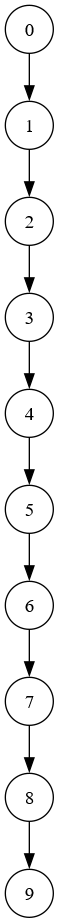
\includegraphics[height=2.7cm,keepaspectratio]{bst.png}
  \caption{BST}
\end{subfigure}
\hfill
\begin{subfigure}[b]{0.16\textwidth}
  \centering
  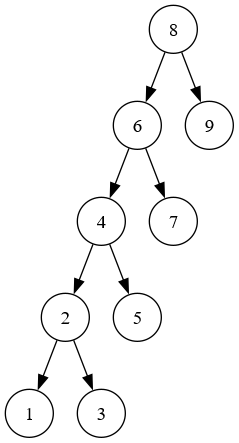
\includegraphics[height=2.7cm,keepaspectratio]{splay.png}
  \caption{Splay Tree}
\end{subfigure}
\hfill
\begin{subfigure}[b]{0.31\textwidth}
  \centering
  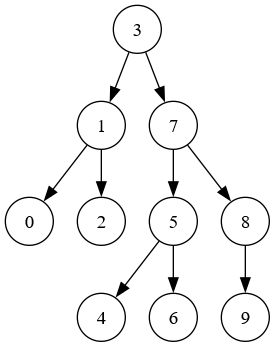
\includegraphics[width=\textwidth,height=2.7cm,keepaspectratio]{avl.png}
  \caption{AVL Tree}
\end{subfigure}
\hfill
\begin{subfigure}[b]{0.31\textwidth}
  \centering
  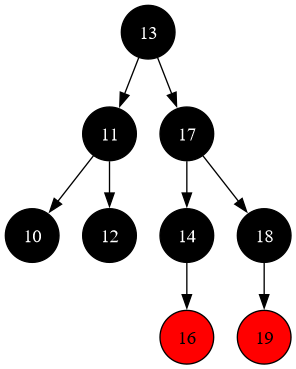
\includegraphics[width=\textwidth,height=2.7cm,keepaspectratio]{rb.png}
  \caption{Red-Black Tree}
\end{subfigure}

\vspace{0.25em}
\begin{subfigure}[b]{0.66\textwidth}
  \centering
  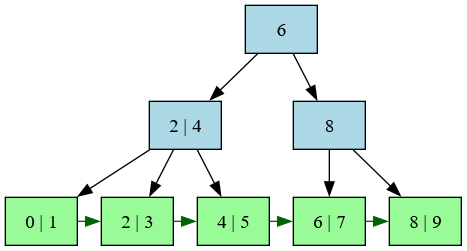
\includegraphics[width=\textwidth,height=2.2cm,keepaspectratio]{b_plus.png}
  \caption{Order-$4$ $\text{B}^+$ Tree with lightblue internal routing nodes and palegreen linked leaves}
\end{subfigure}
\caption{Tree topologies exported by \code{testbench\_figure.c} and rendered via Graphviz.}
\label{fig:topology}
\end{figure}

\subsection{Performance Benchmark Setup and Runtime Table}
The benchmark was evaluated over input sizes $N \in \{1{,}000, 2{,}000, \dots, 50{,}000\}$ with a step size of $1{,}000$, with each data point averaged over $3$ independent repetitions. For the random workload, identical pseudo-random permutations were generated via the Fisher--Yates shuffle to ensure that all five trees process the exact same key sequences. \Cref{tab:runtime_table} reports the measured insertion and deletion times in milliseconds at representative input sizes ($N \in \{1{,}000, 10{,}000, 20{,}000, 30{,}000, 40{,}000, 50{,}000\}$) across all three scenarios.
\vspace{-0.4em}
\begin{table}[H]
\centering
\caption{Execution time comparison in milliseconds across scenarios and input sizes $N$.}
\label{tab:runtime_table}
\renewcommand{\arraystretch}{0.95}
\setlength{\tabcolsep}{4.2pt}
\begin{tabular}{@{}llrrrrrr@{}}
\toprule
\textbf{\color{primary}Scenario} & \textbf{\color{primary}Tree} & \textbf{\color{primary}$N=1{,}000$} & \textbf{\color{primary}$N=10{,}000$} & \textbf{\color{primary}$N=20{,}000$} & \textbf{\color{primary}$N=30{,}000$} & \textbf{\color{primary}$N=40{,}000$} & \textbf{\color{primary}$N=50{,}000$} \\
\midrule
\multirow{5}{*}{\shortstack[l]{Scenario 1: Ordered\\Insertion Time, ms}}
  & BST       & 0.754 & 69.678 & 264.054 & 628.587 & 1129.765 & 1888.738 \\
  & AVL       & 0.183 &  1.702 &   2.992 &   4.424 &    6.619 &    7.833 \\
  & Splay     & 0.036 &  0.250 &   0.581 &   0.514 &    0.736 &    0.778 \\
  & Red-Black & 0.136 &  1.210 &   2.590 &   3.873 &    5.615 &    6.942 \\
  & $\text{B}^+$ Tree & 0.247 &  2.972 &   4.557 &   6.809 &    8.891 &   12.355 \\
\midrule
\multirow{5}{*}{\shortstack[l]{Scenario 1: Ordered\\Deletion Time, ms}}
  & BST       & 0.016 &  0.171 &   0.217 &   0.301 &    0.399 &    0.599 \\
  & AVL       & 0.130 &  1.069 &   2.221 &   4.712 &    5.656 &    8.075 \\
  & Splay     & 0.044 &  0.227 &   0.449 &   0.735 &    0.929 &    1.177 \\
  & Red-Black & 0.054 &  0.485 &   1.021 &   1.609 &    2.931 &    3.319 \\
  & $\text{B}^+$ Tree & 0.159 &  1.332 &   3.167 &   6.714 &    9.338 &   12.306 \\
\midrule
\multirow{5}{*}{\shortstack[l]{Scenario 2: Reverse\\Deletion Time, ms}}
  & BST       & 0.684 & 63.698 & 251.397 & 590.257 & 1139.824 & 1777.648 \\
  & AVL       & 0.121 &  1.130 &   2.412 &   4.375 &    5.891 &    8.341 \\
  & Splay     & 0.018 &  0.110 &   0.227 &   0.336 &    0.391 &    0.646 \\
  & Red-Black & 0.071 &  0.522 &   1.059 &   2.438 &    2.246 &    3.177 \\
  & $\text{B}^+$ Tree & 0.157 &  1.281 &   3.182 &   5.975 &    6.615 &    8.095 \\
\midrule
\multirow{5}{*}{\shortstack[l]{Scenario 3: Random\\Insertion Time, ms}}
  & BST       & 0.090 &  0.843 &   1.941 &   3.838 &    4.015 &    5.524 \\
  & AVL       & 0.334 &  2.155 &   4.478 &   9.397 &   10.925 &   12.785 \\
  & Splay     & 0.166 &  1.858 &   3.941 &   7.184 &    8.619 &   10.446 \\
  & Red-Black & 0.179 &  1.588 &   3.563 &   5.608 &    7.387 &   10.409 \\
  & $\text{B}^+$ Tree & 0.276 &  3.000 &   7.625 &  12.549 &   16.264 &   19.595 \\
\midrule
\multirow{5}{*}{\shortstack[l]{Scenario 3: Random\\Deletion Time, ms}}
  & BST       & 0.074 &  0.764 &   1.753 &   2.985 &    4.417 &    5.359 \\
  & AVL       & 0.276 &  1.851 &   4.748 &   7.178 &   10.779 &   13.538 \\
  & Splay     & 0.198 &  1.371 &   3.342 &   6.337 &    7.656 &   10.079 \\
  & Red-Black & 0.239 &  1.095 &   2.456 &   4.473 &    5.650 &    7.303 \\
  & $\text{B}^+$ Tree & 0.235 &  2.548 &   6.142 &  11.828 &   16.430 &   20.871 \\
\bottomrule
\end{tabular}
\end{table}

\vspace{-0.5em}
\subsection{Runtime Plots vs.\ Input Size}
\Cref{fig:ordered_plots,fig:reverse_plots,fig:random_plots} present the six runtime curves generated by \code{visualization.py} across $N \in [1{,}000, 50{,}000]$.

\vspace{-0.5em}
\begin{figure}[H]
\centering
\captionsetup[subfigure]{skip=2pt}
\begin{subfigure}[b]{0.475\textwidth}
  \centering
  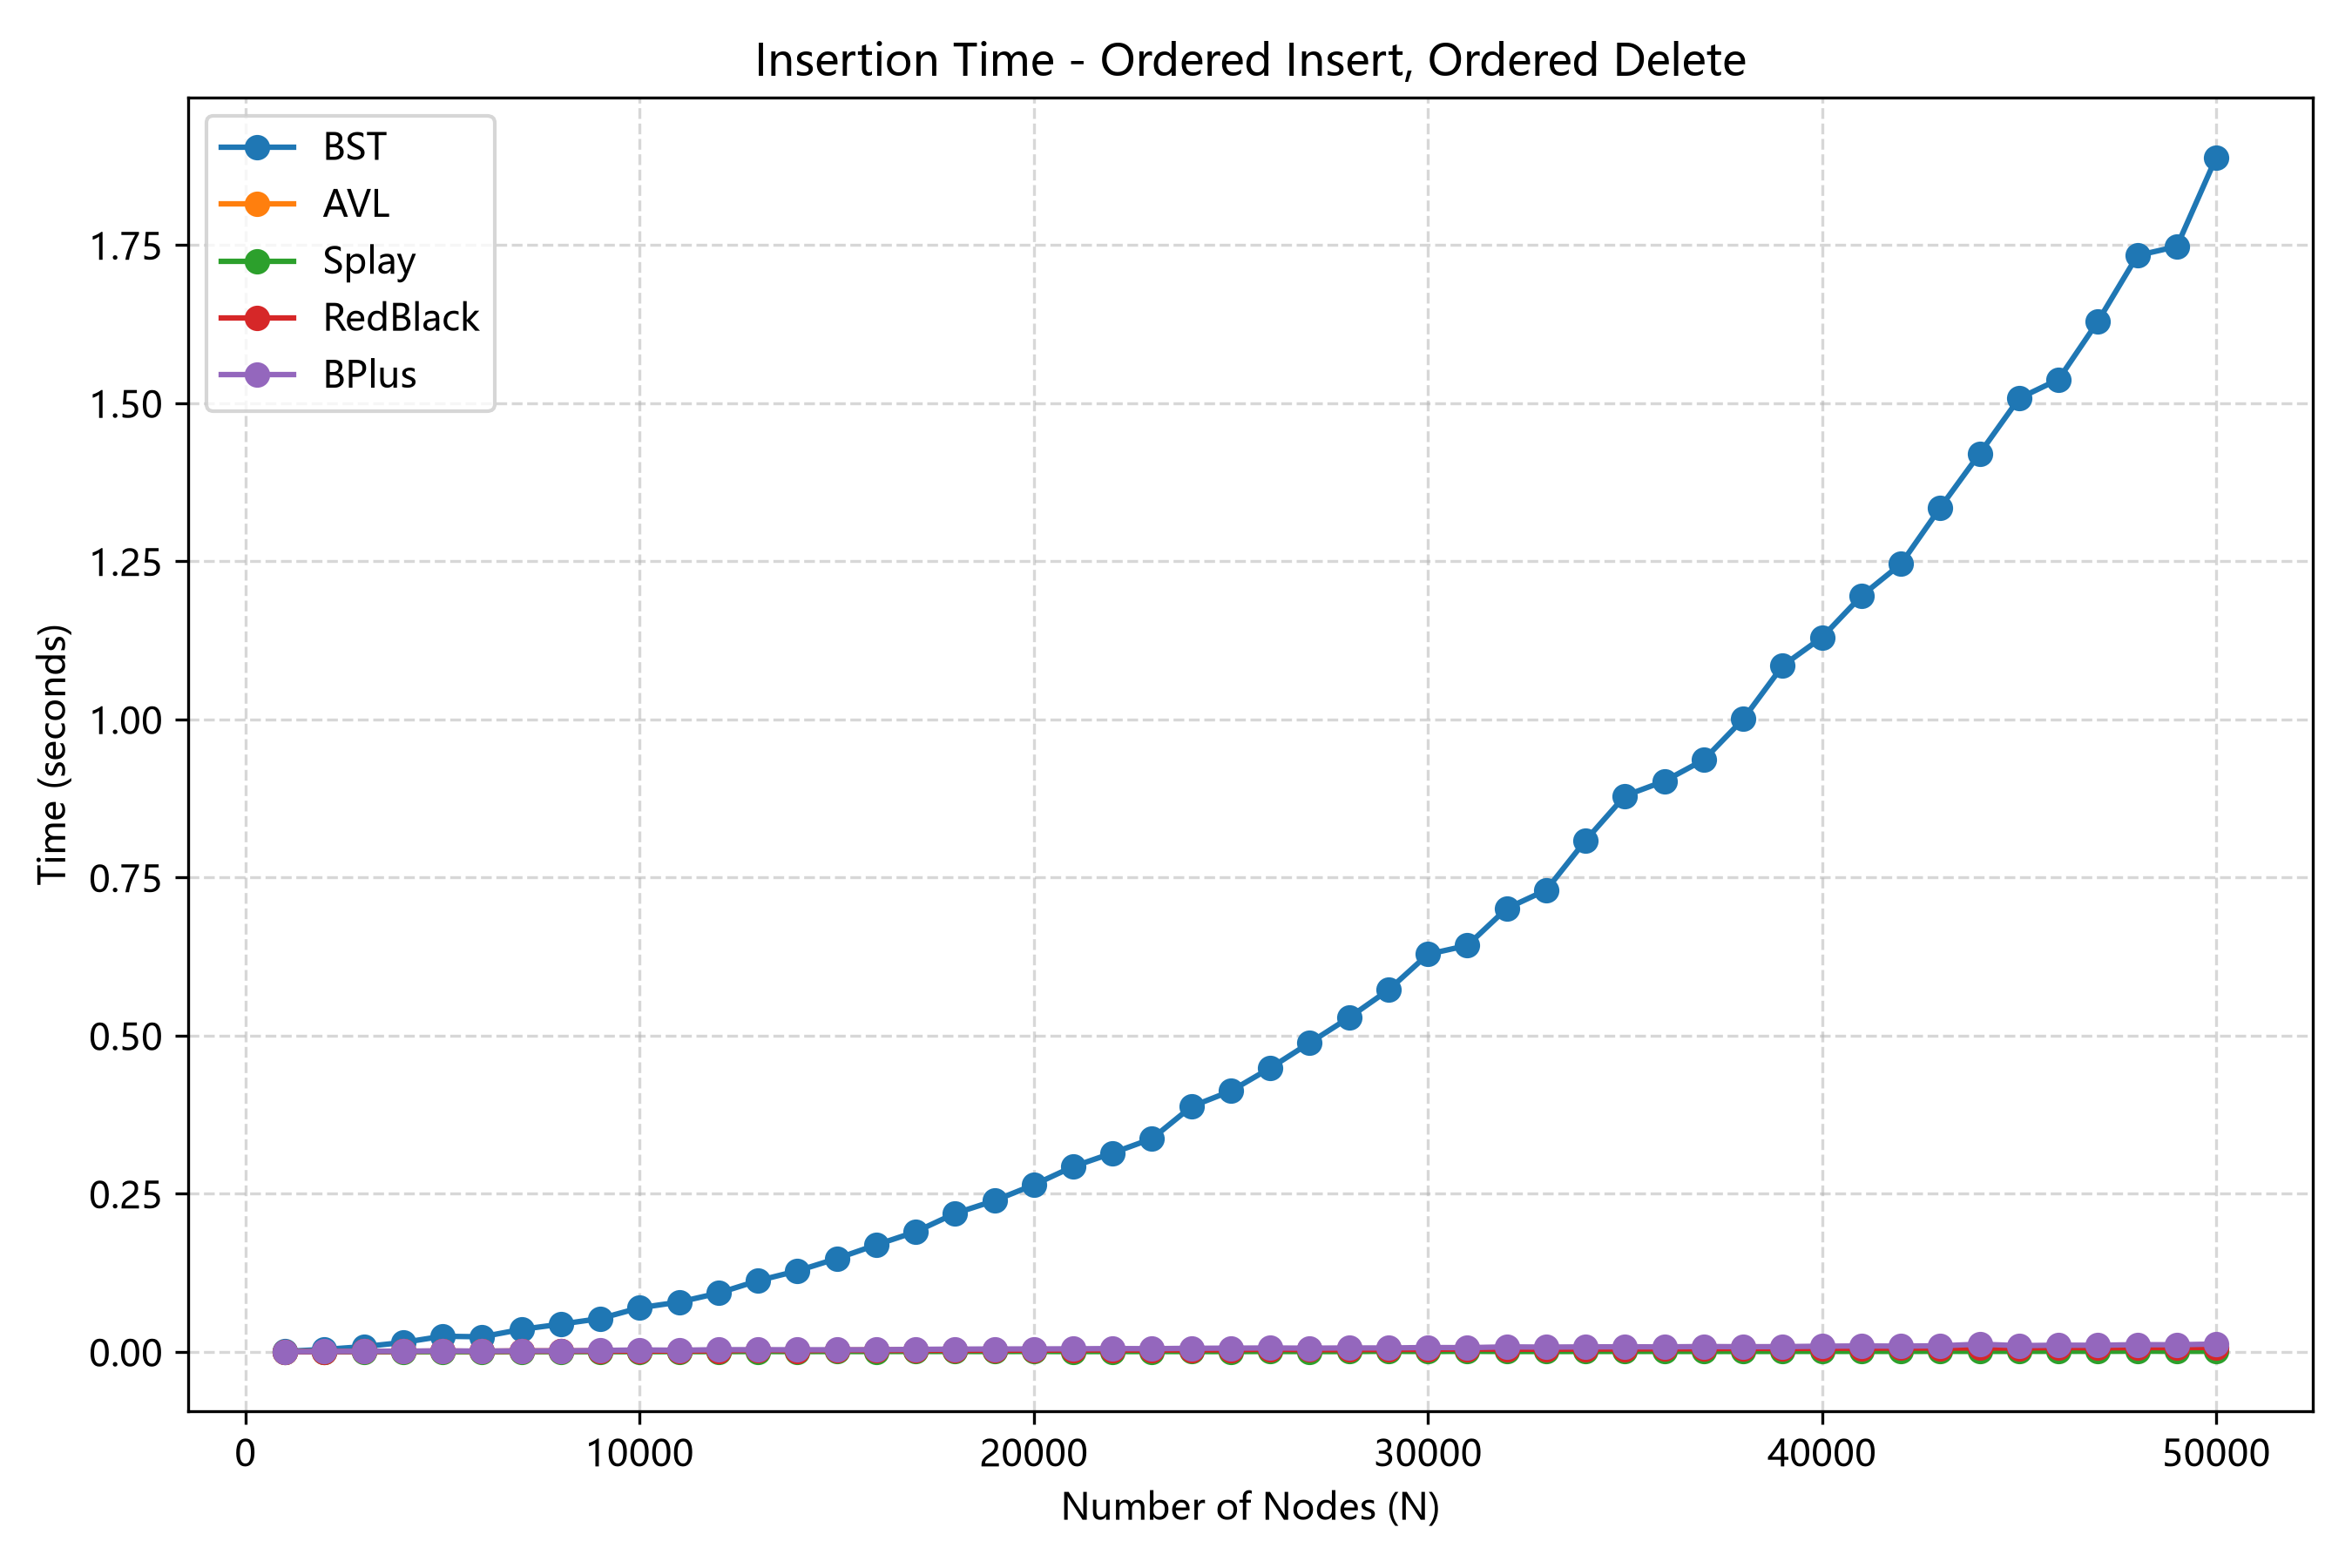
\includegraphics[width=\textwidth]{ordered_insert_seconds.png}
  \caption{Ordered insertion time}
  \label{fig:ordered_ins}
\end{subfigure}
\hfill
\begin{subfigure}[b]{0.475\textwidth}
  \centering
  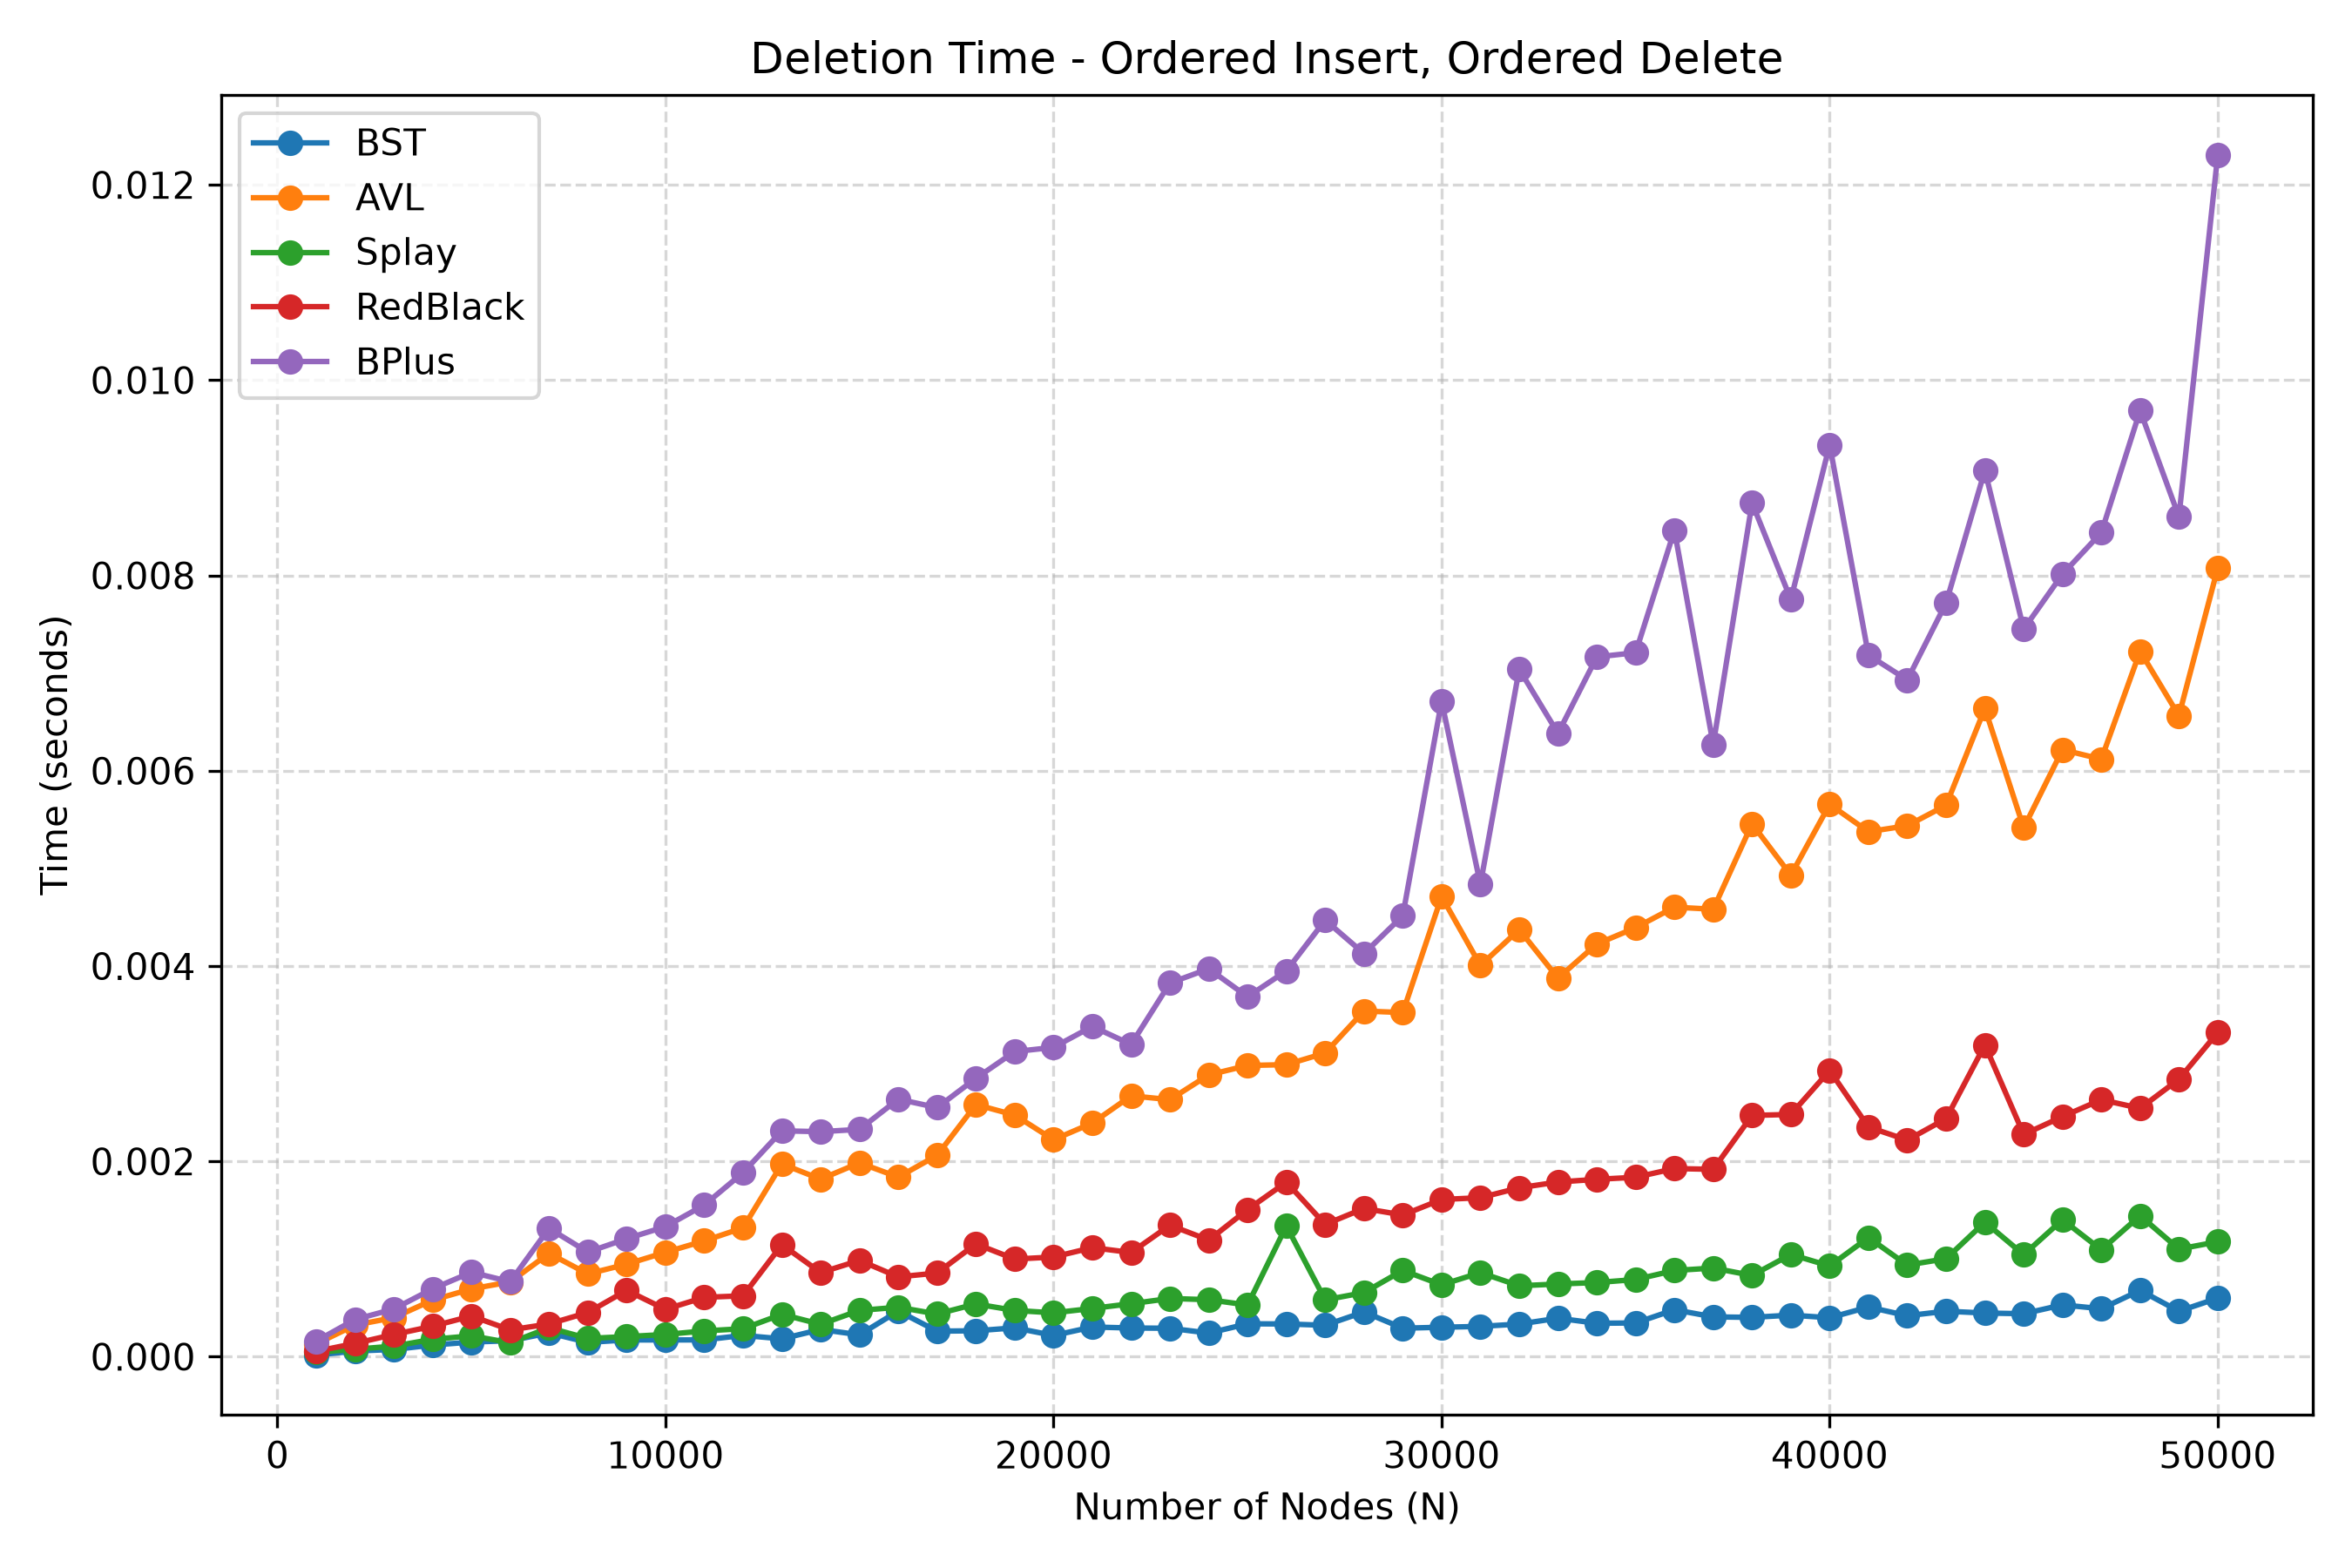
\includegraphics[width=\textwidth]{ordered_delete_seconds.png}
  \caption{Ordered deletion time}
  \label{fig:ordered_del}
\end{subfigure}
\caption{Scenario 1: Increasing-order insertion followed by increasing-order deletion.}
\label{fig:ordered_plots}
\end{figure}

\begin{figure}[H]
\centering
\begin{subfigure}[b]{0.485\textwidth}
  \centering
  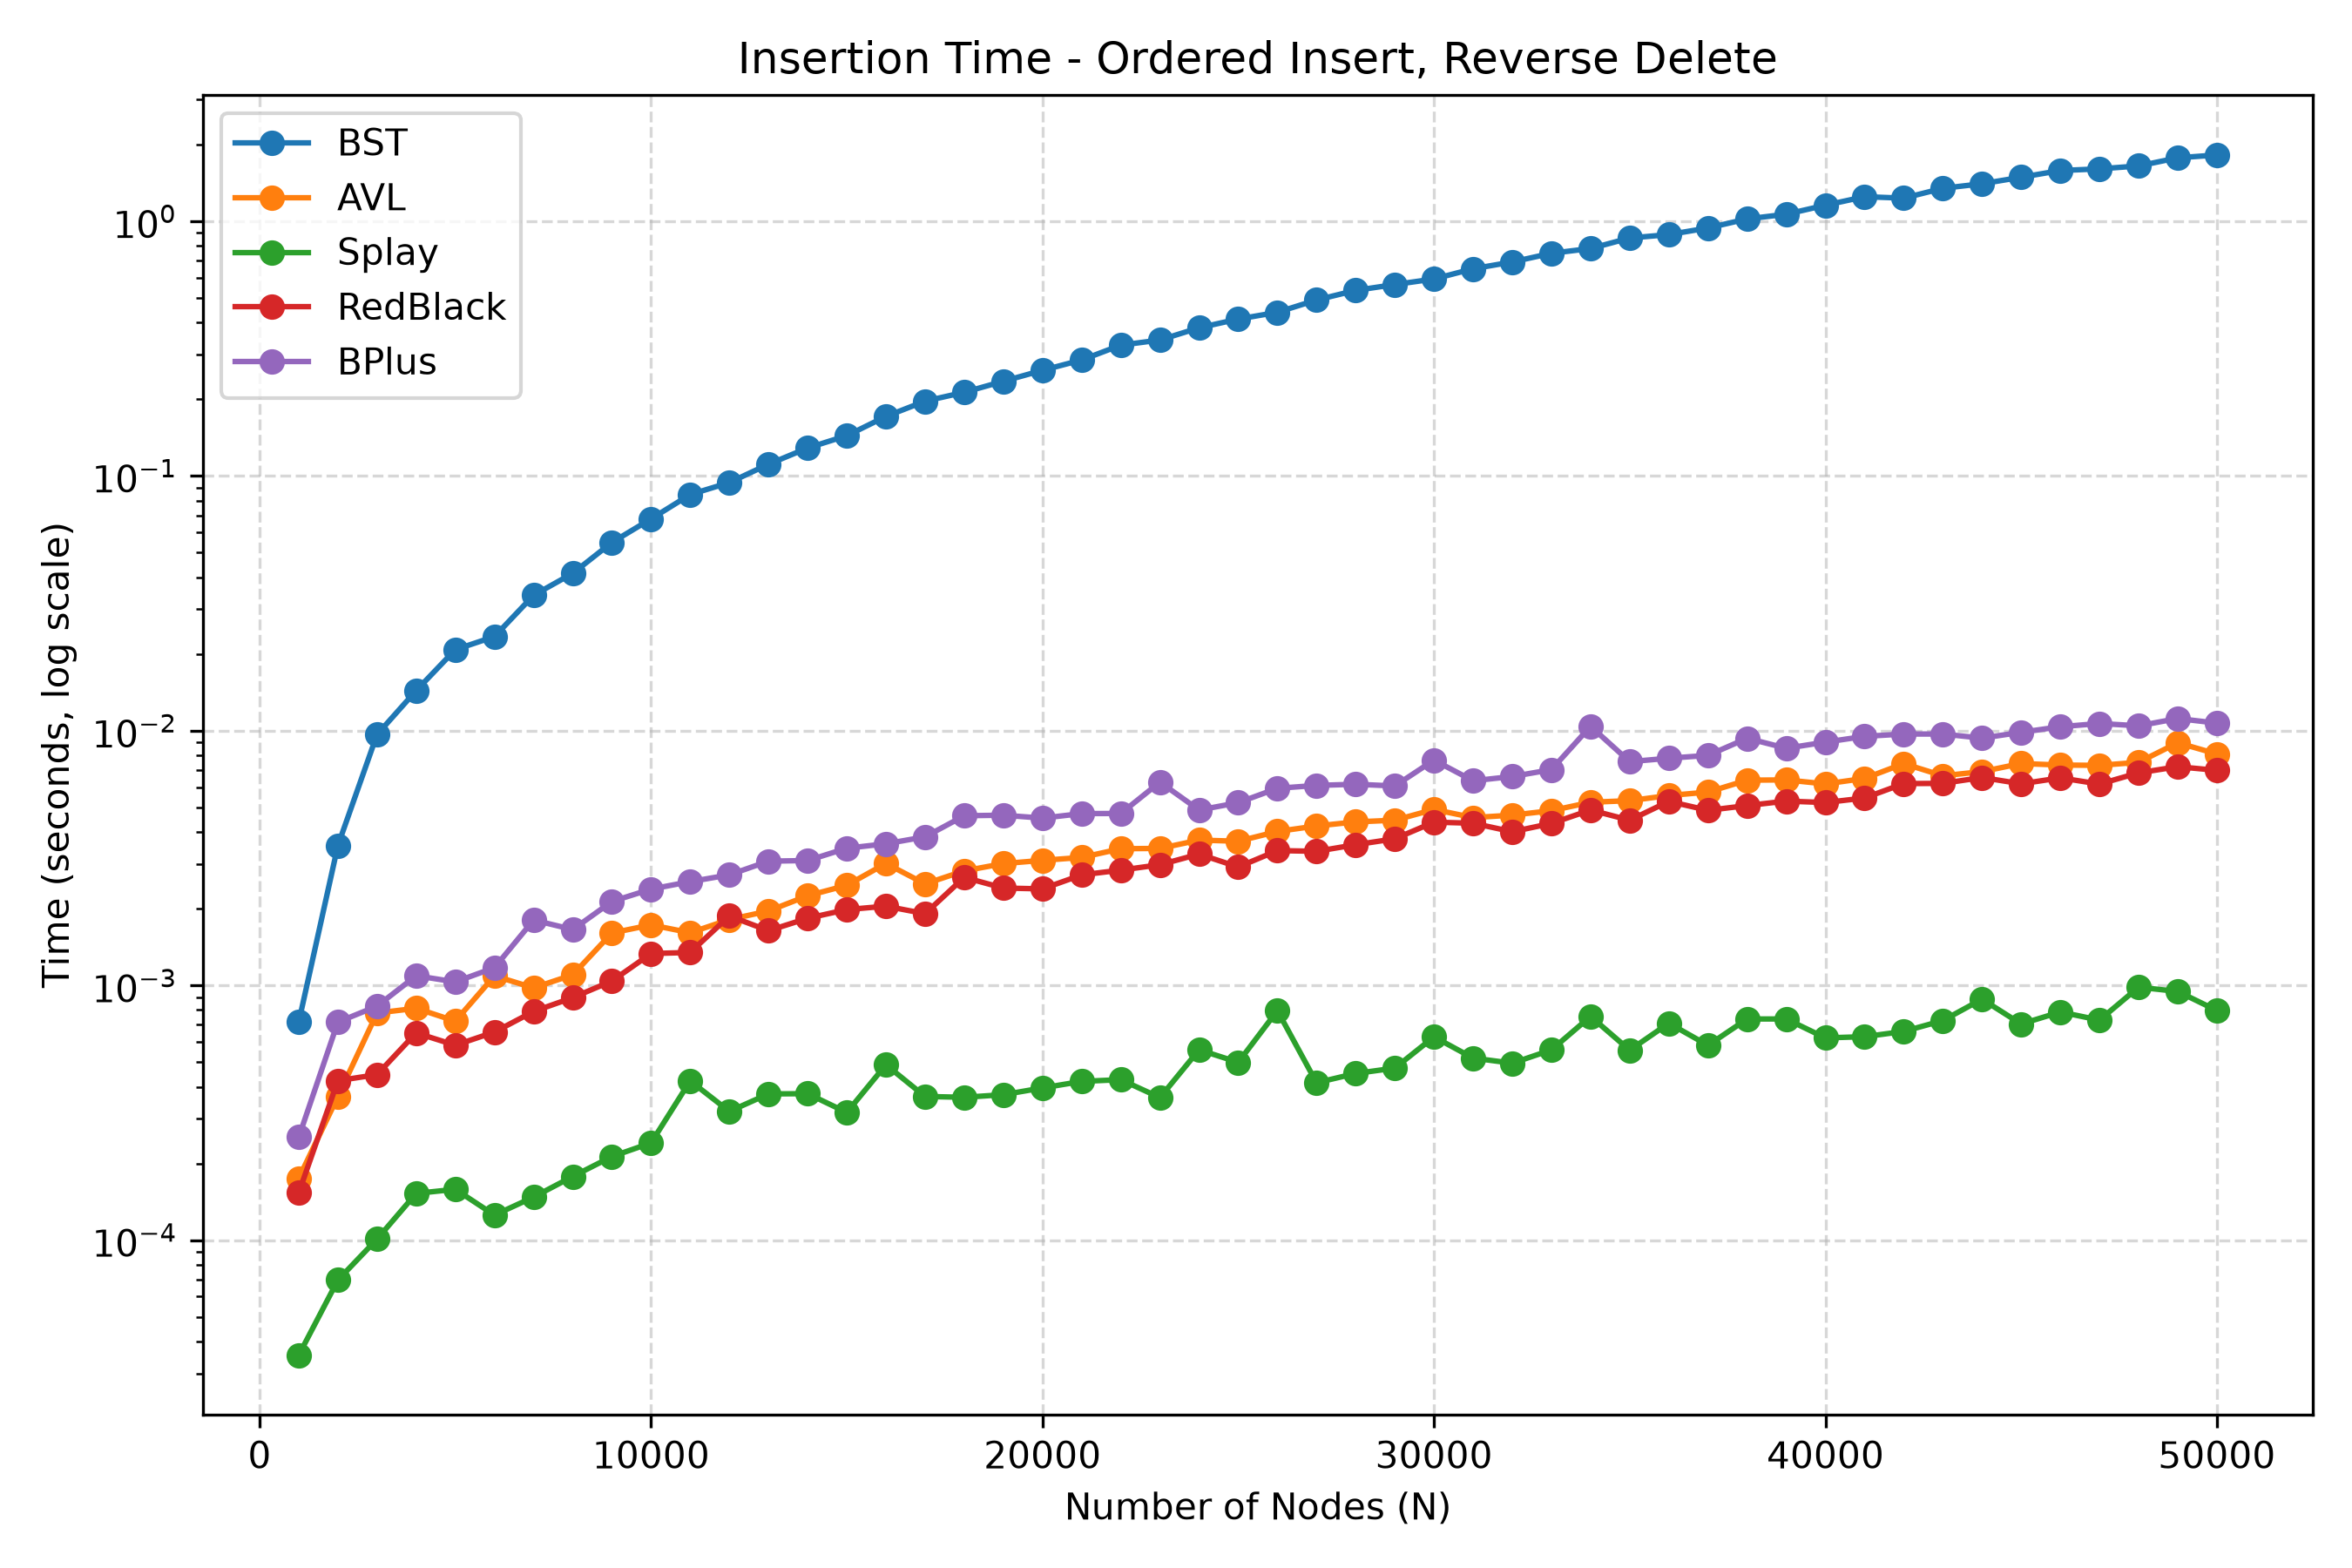
\includegraphics[width=\textwidth]{ordered_reverse_insert_seconds.png}
  \caption{Ordered insertion time}
  \label{fig:rev_ins}
\end{subfigure}
\hfill
\begin{subfigure}[b]{0.485\textwidth}
  \centering
  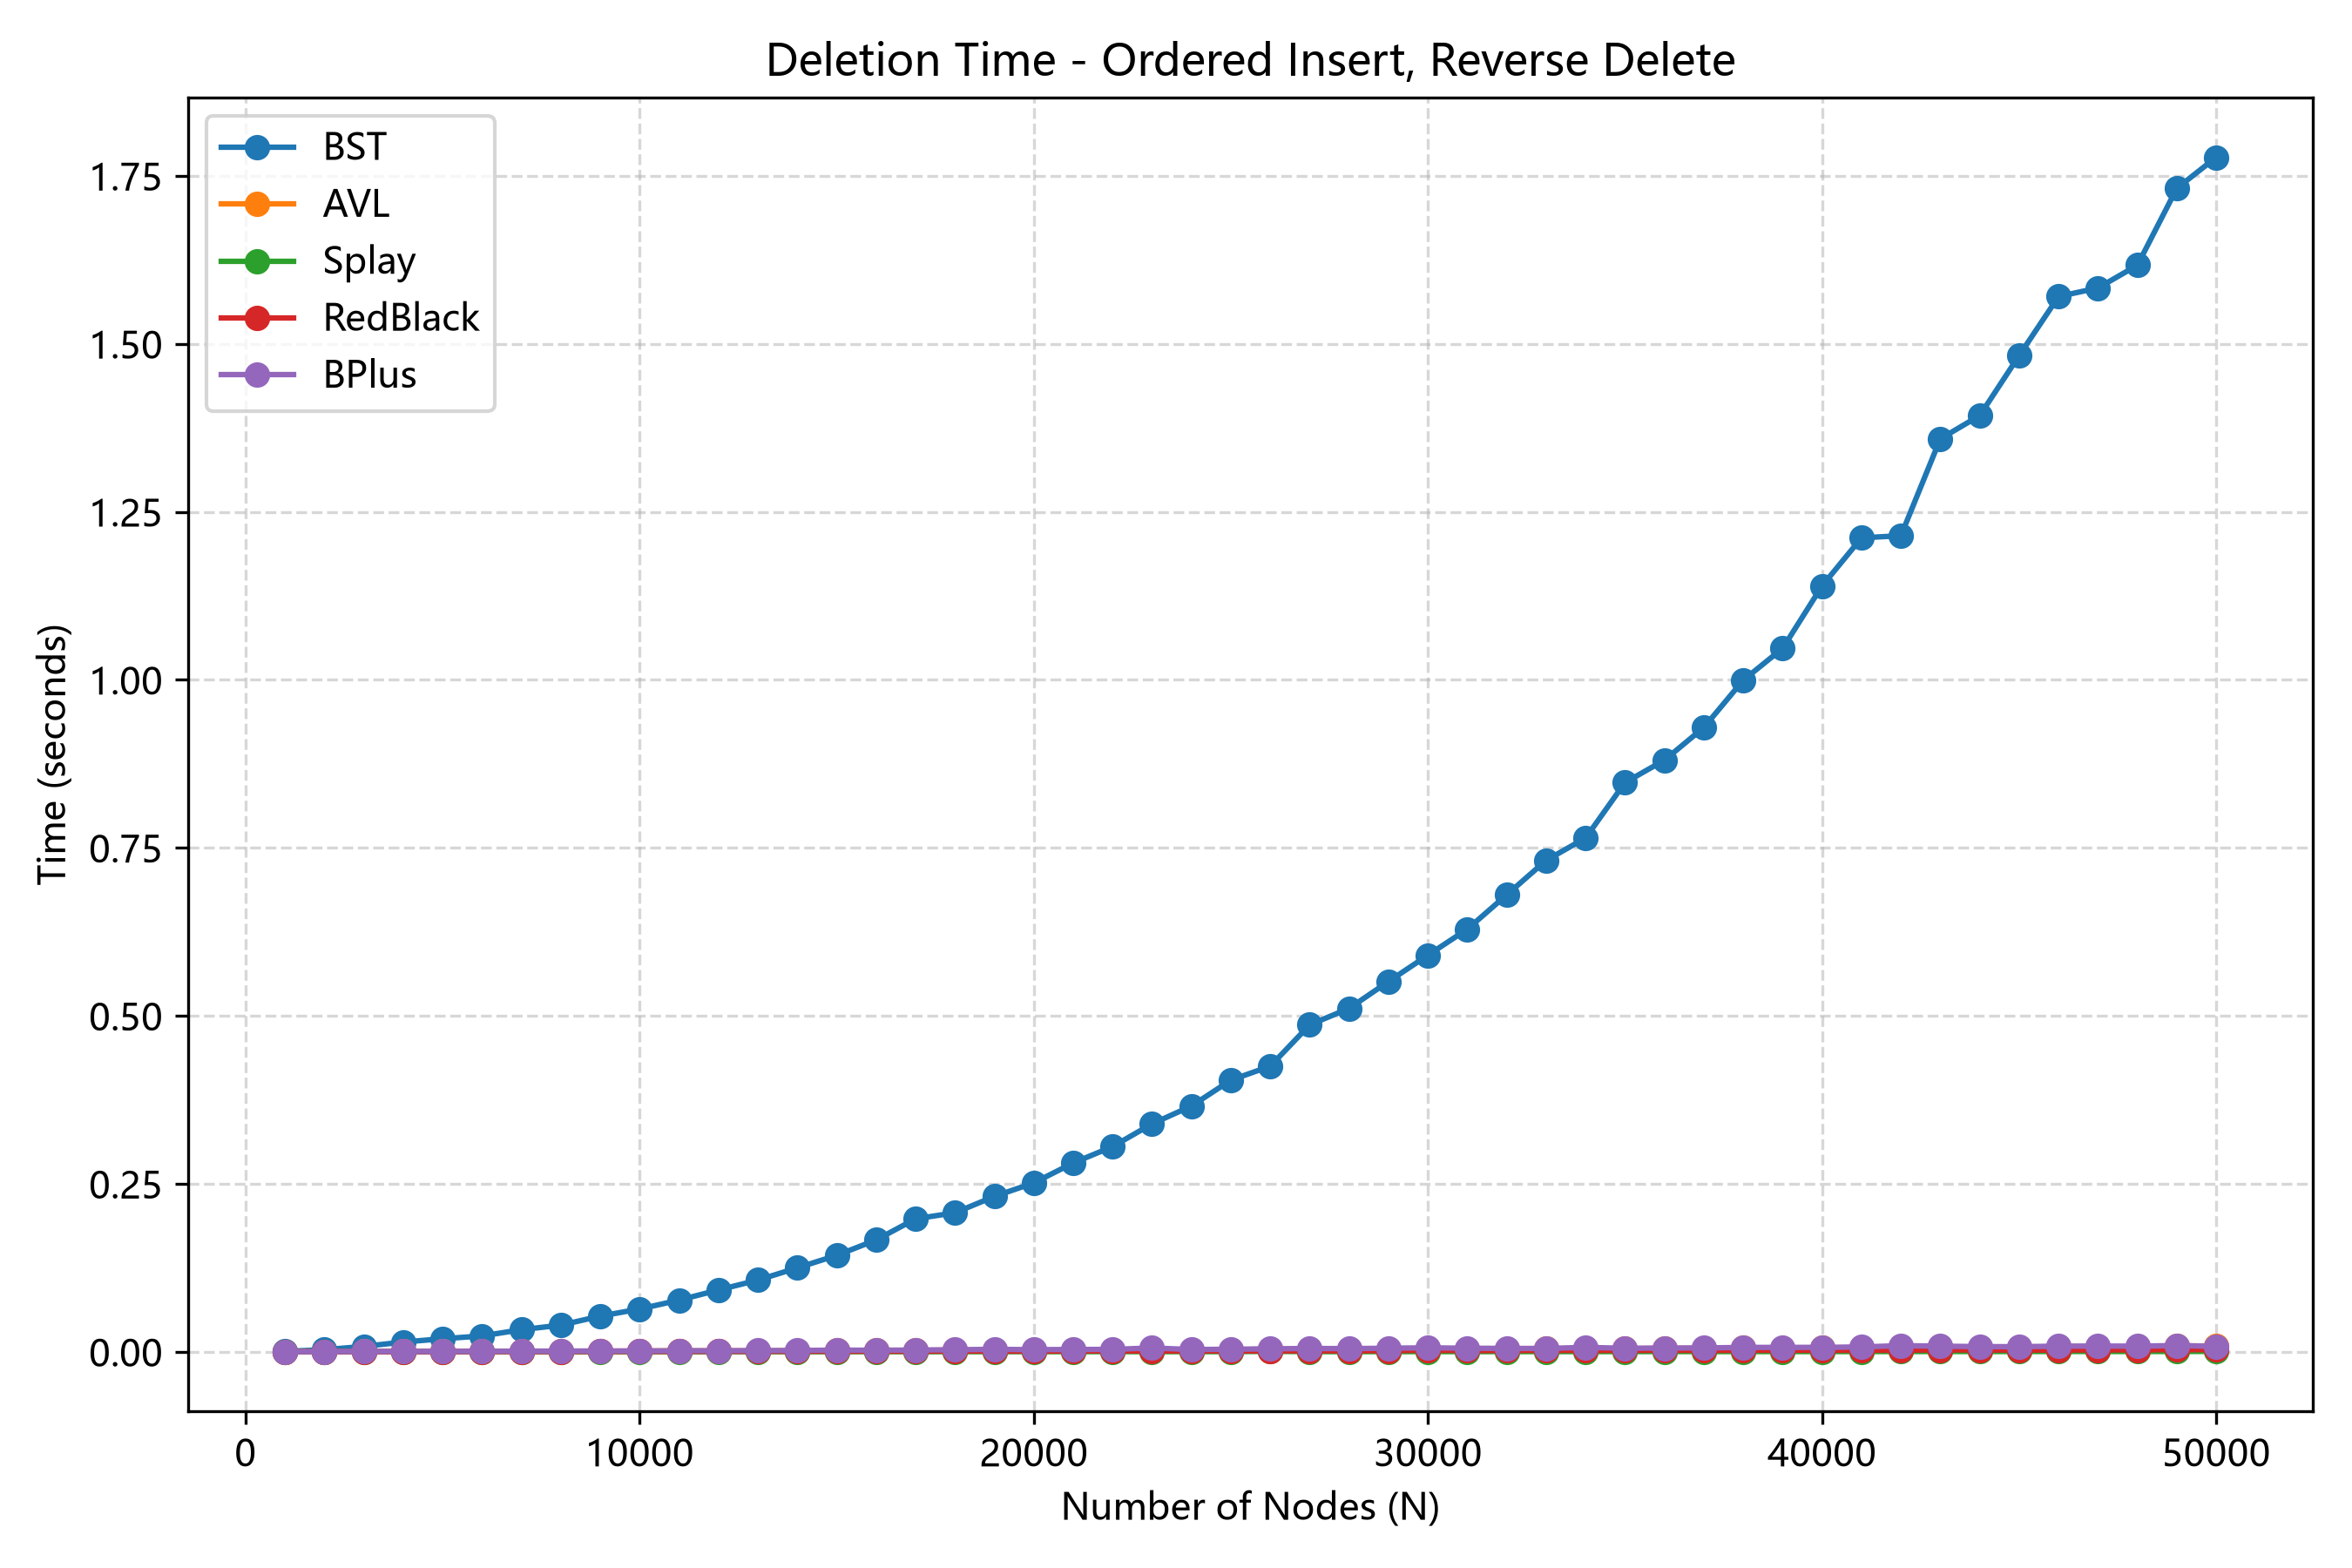
\includegraphics[width=\textwidth]{ordered_reverse_delete_seconds.png}
  \caption{Reverse deletion time}
  \label{fig:rev_del}
\end{subfigure}
\caption{Scenario 2: Increasing-order insertion followed by reverse-order deletion.}
\label{fig:reverse_plots}
\end{figure}

\begin{figure}[H]
\centering
\begin{subfigure}[b]{0.485\textwidth}
  \centering
  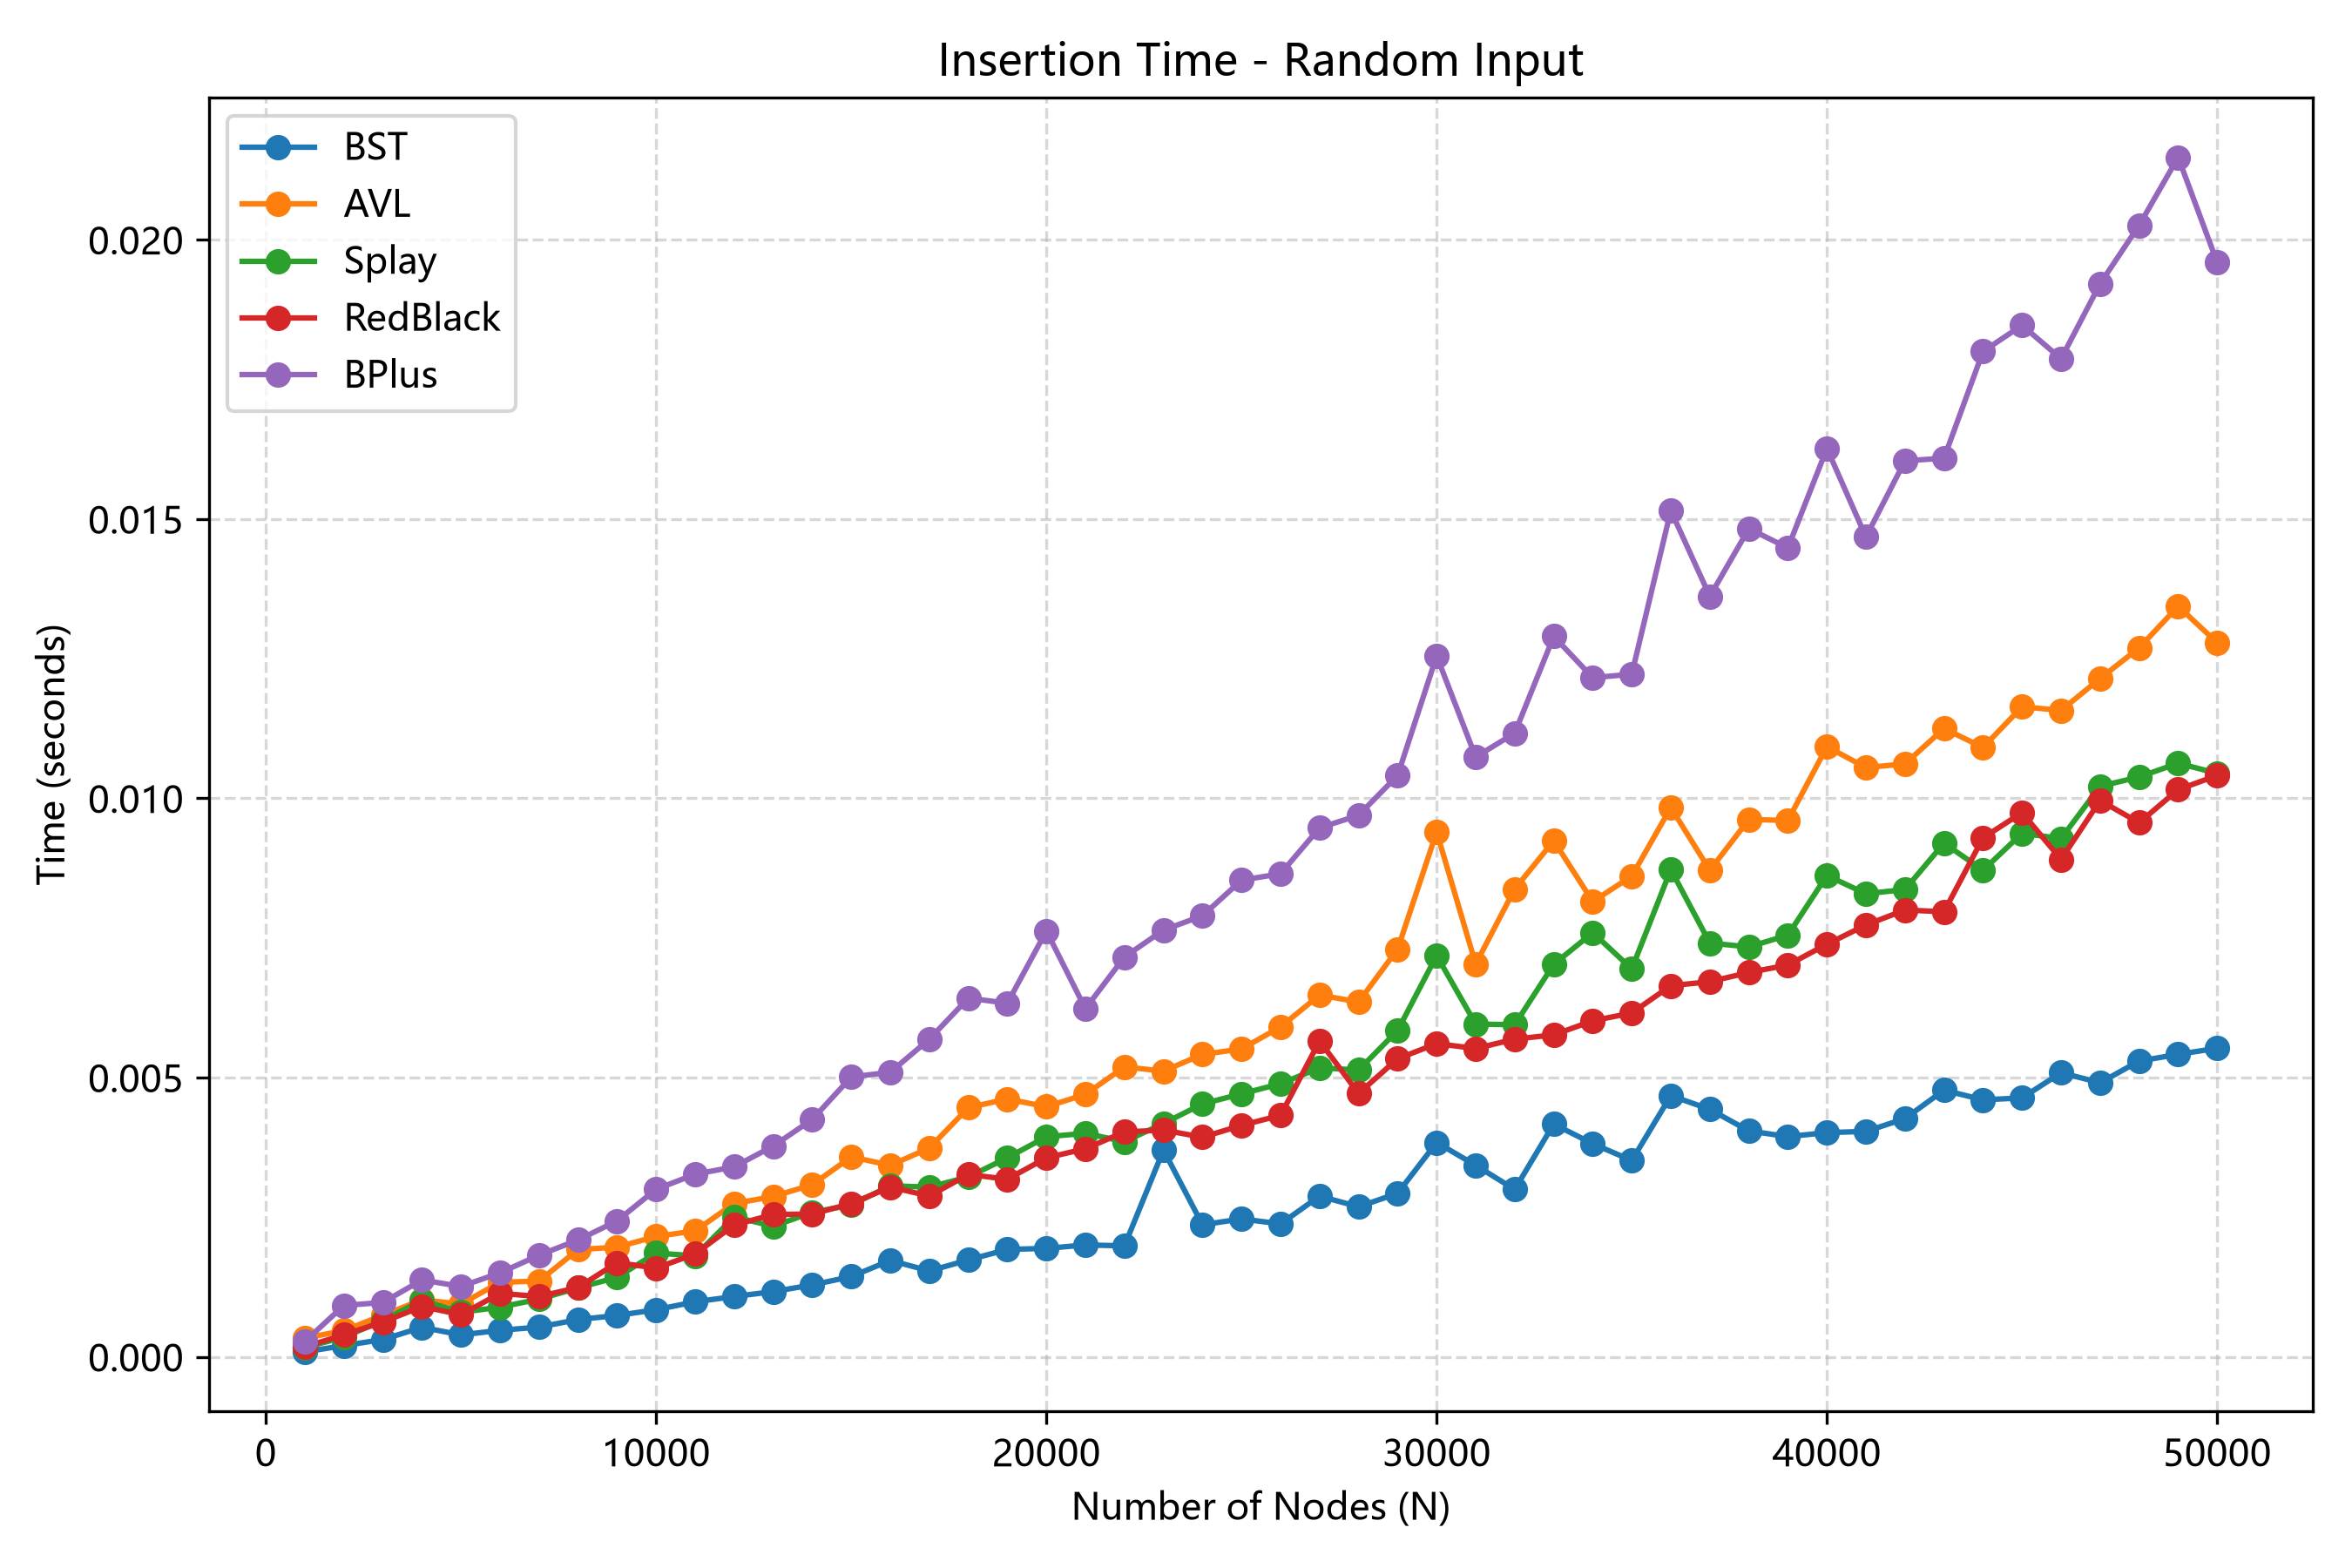
\includegraphics[width=\textwidth]{random_insert_seconds.png}
  \caption{Random insertion time}
  \label{fig:rand_ins}
\end{subfigure}
\hfill
\begin{subfigure}[b]{0.485\textwidth}
  \centering
  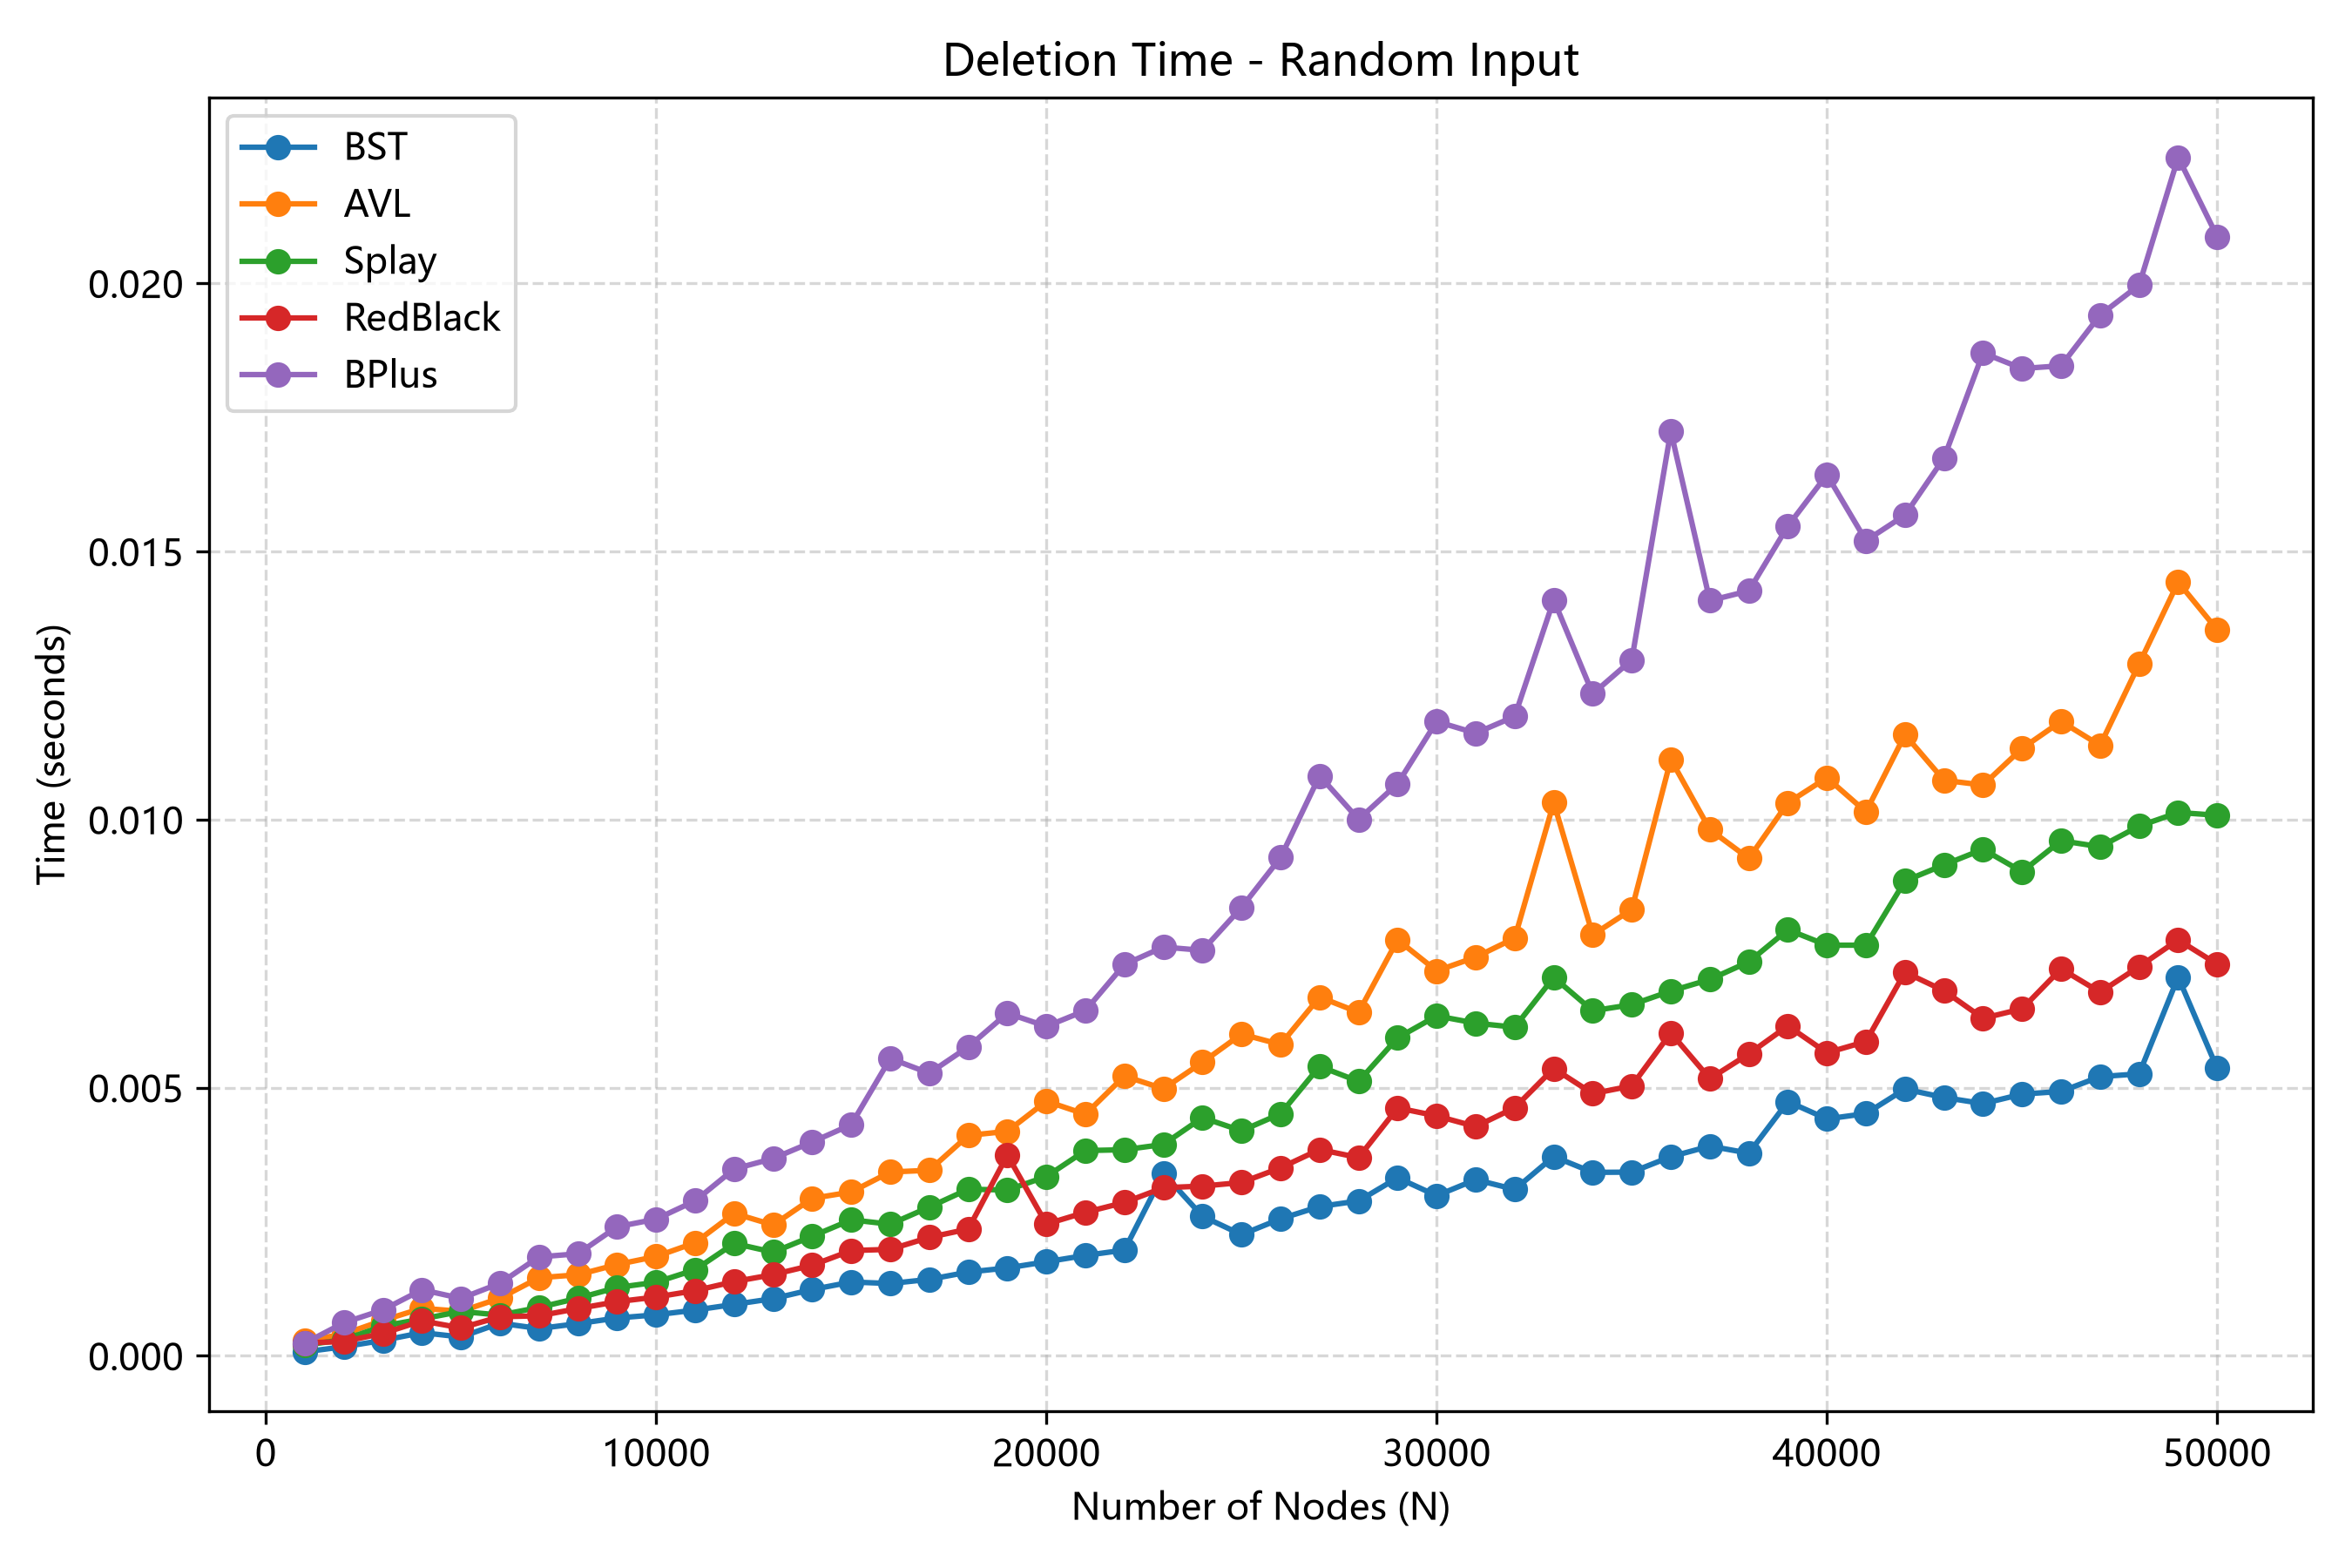
\includegraphics[width=\textwidth]{random_delete_seconds.png}
  \caption{Random deletion time}
  \label{fig:rand_del}
\end{subfigure}
\caption{Scenario 3: Uniform random-order insertion followed by random-order deletion.}
\label{fig:random_plots}
\end{figure}

\clearpage

% ============================================================
%  CHAPTER 4: ANALYSIS AND COMMENTS
% ============================================================
\section{Analysis and Comments}

\subsection{Time and Space Complexity Analysis}
\Cref{tab:complexities} summarizes the theoretical time and space complexities of a single dictionary operation and a sequence of $N$ operations for all five structures.

\begin{table}[H]
\centering
\caption{Theoretical asymptotic time and space complexities.}
\label{tab:complexities}
\setlength{\tabcolsep}{3.5pt}
\begin{tabular}{@{}lcccc@{}}
\toprule
\textbf{\color{primary}Structure} & \textbf{\color{primary}Average Op} & \textbf{\color{primary}Worst-Case Op} & \textbf{\color{primary}Sorted Ins + Same Del} & \textbf{\color{primary}Sorted Ins + Rev Del} \\
\midrule
Unbalanced BST   & $\Theta(\log N)$ & $\Theta(N)$               & $\Theta(N^2)$ ins / $\Theta(N)$ del & $\Theta(N^2)$ ins / $\Theta(N^2)$ del \\
AVL Tree         & $\Theta(\log N)$ & $\Theta(\log N)$          & $\Theta(N\log N)$                   & $\Theta(N\log N)$                     \\
Splay Tree       & $\Theta(\log N)$ amort. & $\Theta(N)$ single & $\Theta(N)$ ins / $\Theta(N)$ del   & $\Theta(N)$ ins / $\Theta(N)$ del     \\
Red-Black Tree   & $\Theta(\log N)$ & $\Theta(\log N)$          & $\Theta(N\log N)$                   & $\Theta(N\log N)$                     \\
Order-$4$ $\text{B}^+$ Tree & $\Theta(\log N)$ & $\Theta(\log N)$ & $\Theta(N\log N)$                   & $\Theta(N\log N)$                     \\
\bottomrule
\end{tabular}
\end{table}

\paragraph{Space Complexity.}
Every dynamic tree stores $O(N)$ nodes in heap memory. Specifically:
\begin{itemize}
  \item \textbf{BST and Splay Tree} require the minimal node size of $24$ bytes on 64-bit targets, comprising one integer key and two child pointers, with $O(1)$ auxiliary stack space for our iterative BST and $O(H)$ recursion stack space for Splay.
  \item \textbf{AVL Tree} adds two integer fields \code{height} and \code{BF}, taking $32$ bytes per node and $O(\log N)$ recursion stack space.
  \item \textbf{Red-Black Tree} adds a \code{color} field and a \code{parent} pointer for $40$ bytes per node, while its fix-up loops are purely iterative and use $O(1)$ auxiliary space after node insertion.
  \item \textbf{$\text{B}^+$ Tree} allocates dynamic key and child pointer arrays \code{keys[4]} and \code{children[5]} per node, consuming more heap allocations per key for small order $M=4$, though with reduced tree depth $\log_{2\dots 4} N$.
\end{itemize}

\subsection{Workload-Specific Empirical Behavior}

\subsubsection{Asymmetry of Unbalanced BST Under Ordered vs.\ Reverse Deletion}
One of the most striking phenomena in \cref{fig:ordered_plots,fig:reverse_plots} is the dramatic difference in Unbalanced BST deletion time between Scenario 1 and Scenario 2:

\begin{insightbox}{Key Finding 1: Why BST Ordered Deletion Takes $\Theta(N)$ While Reverse Deletion Takes $\Theta(N^2)$}
\begin{itemize}
  \item \textbf{Ordered Insertion, $\Theta(N^2)$ total:} Inserting $0, 1, \dots, N-1$ appends each new key to the rightmost leaf of a right-skewed chain. The $k$-th insertion traverses $k$ nodes, yielding $\sum_{k=0}^{N-1} k = \frac{N(N-1)}{2} = \Theta(N^2)$ comparisons. Empirically, when $N$ increases $5\times$ from $10{,}000$ to $50{,}000$, BST insertion time increases by $1888.74 / 69.68 \approx 27.1\times$, which closely matches the theoretical factor $5^2 = 25$ together with cache-miss amplification.
  \item \textbf{Scenario 1 --- Increasing Deletion, $\Theta(N)$ total:} In a right-skewed chain $0 \to 1 \to \dots \to N-1$, the smallest element is always the \textbf{current root}. Deleting keys in increasing order $0, 1, \dots, N-1$ repeatedly removes the root node in $O(1)$ time by advancing $\code{root} \gets \code{root->Right}$ without traversing the chain. Thus $N$ deletions take $\Theta(N)$ total time, reaching only $0.60\,\text{ms}$ at $N=50{,}000$ and making BST the fastest structure in \cref{fig:ordered_del}.
  \item \textbf{Scenario 2 --- Reverse Deletion, $\Theta(N^2)$ total:} Deleting keys in decreasing order $N-1, N-2, \dots, 0$ always targets the \textbf{deepest leaf} at the bottom of the right chain. The $k$-th deletion must traverse $N-k$ nodes from the root, resulting in $\sum_{k=1}^{N} (N-k) = \Theta(N^2)$ total time, or $1.78\,\text{s}$ at $N=50{,}000$ in \cref{fig:rev_del}.
\end{itemize}
\end{insightbox}

\subsubsection{Sequential Locality Advantage of Splay Trees}
Across both Scenario 1 and Scenario 2, the \textbf{Splay Tree} is by far the fastest structure for sorted insertions and reverse deletions, taking only $0.78\,\text{ms}$ and $0.65\,\text{ms}$ at $N=50{,}000$, which is nearly an order of magnitude faster than Red-Black and AVL Trees.

\begin{insightbox}{Key Finding 2: $\Theta(N)$ Sequential Access Performance of Splay Trees}
\begin{itemize}
  \item \textbf{Increasing Insertion, $\Theta(N)$ total:} Because \code{insertSplay} splays each newly inserted key $k$ to the root via split, when $k+1$ arrives, the root already holds the largest existing key $k$ and has an empty right subtree. Thus \code{findSplay(root, k+1)} immediately terminates in $O(1)$ time at the root, and \code{insertSplay} attaches $k+1$ as the new root with $k$ as its left child in $O(1)$ time. This constructs a left-skewed spine in $\Theta(N)$ total time, as shown in \cref{fig:topology}b.
  \item \textbf{Reverse Deletion, $\Theta(N)$ total:} At the end of increasing insertion, the tree is a left chain rooted at $N-1$ with parent-to-left-child order $N-1 \to N-2 \to \dots \to 0$. Deleting in reverse order $N-1, N-2, \dots, 0$ always deletes the current root in $O(1)$ time.
  \item \textbf{Increasing Deletion, $\Theta(N)$ amortized:} Even when deleting $0$ from depth $N-1$ on the left spine, the first \code{findSplay(root, 0)} performs a sequence of \emph{zig-zig} rotations that halves the depth of every node along the spine, folding the chain into a shallow tree so subsequent deletions of $1, 2, \dots$ take $O(1)$ amortized time~\cite{ads_slides2026}, finishing in $1.18\,\text{ms}$ at $N=50{,}000$.
\end{itemize}
\end{insightbox}

\subsubsection{Trade-offs Among Balanced Trees under Random Workloads}
In Scenario 3, shown in \cref{fig:random_plots}, random permutations eliminate adversarial skew, yielding the runtime ranking $\textbf{BST} < \textbf{Red-Black} < \textbf{Splay} < \textbf{AVL} < \textbf{B}^+\textbf{ Tree}$ at $N=50{,}000$:
\begin{enumerate}[label=\textbf{\color{primary}\arabic*.}]
  \item \textbf{Unbalanced BST:} A random BST has expected depth $2\ln N \approx 1.39\log_2 N$ and performs zero rotations or metadata updates, making it the fastest structure when input randomness is guaranteed.
  \item \textbf{Red-Black Tree vs.\ AVL Tree:} At $N=50{,}000$, the Red-Black Tree takes $10.41\,\text{ms}$ for insertion and $7.30\,\text{ms}$ for deletion, whereas the AVL Tree takes $12.79\,\text{ms}$ and $13.54\,\text{ms}$. Both maintain $O(\log N)$ height, but Red-Black Trees consistently outperform AVL Trees by $20\%\text{--}45\%$ on both ordered and random updates. While AVL deletion may trigger $\Theta(\log N)$ rotations propagating to the root, Red-Black insertion requires at most $2$ rotations and Red-Black deletion requires at most $3$ rotations, resolving most imbalances via fast color flips.
  \item \textbf{Splay Tree:} Under uniform random access, splaying loses its locality advantage and pays constant-factor rotation overhead on every lookup, performing comparably to Red-Black on insertion and slightly slower on deletion.
  \item \textbf{$\text{B}^+$ Tree:} The order-$4$ $\text{B}^+$ Tree is the slowest in our benchmarks. Each split, borrow, or merge allocates dynamic arrays, shifts elements linearly inside \code{keys[]} and \code{children[]}, and invokes \code{refreshBPlusAncestors} to walk down \code{children[0]} and update separator keys, incurring much higher constant-factor overhead per operation than binary tree pointer rotations.
\end{enumerate}

\subsection{Further Possible Improvements}
Based on our implementation and profiling results, several engineering improvements can be pursued:
\begin{enumerate}[label=\textbf{\color{primary}\arabic*.}]
  \item \textbf{Eliminating Redundant Separator Updates in $\text{B}^+$ Tree:} Currently, \code{refreshBPlusAncestors} invokes \code{firstBPlusKey} on every child of every ancestor after each update. Caching the minimum key in each node would reduce per-update overhead by a large constant factor.
  \item \textbf{Using Fixed-Size Arrays in $\text{B}^+$ Tree Nodes:} Replacing per-node \code{malloc} calls for \code{keys} and \code{children} with fixed-size arrays \code{int keys[M]} and \code{BPlusTreeNode* children[M+1]} inside the node struct would avoid repeated heap allocations on every node creation.
  \item \textbf{Top-Down Splaying and Memory Pool Allocation:} Replacing recursive splaying with iterative top-down splaying would remove recursion stack overhead, and using a pre-allocated node memory pool (\textbf{from OOP Lab 7 last semester}) across all trees would isolate tree algorithm cost from operating-system \code{malloc} and \code{free} overhead.
\end{enumerate}

\clearpage

% ============================================================
%  AUTHOR LIST, DECLARATION, AND REFERENCES
% ============================================================
\section*{Author List and Declaration}
\addcontentsline{toc}{section}{Author List and Declaration}

\subsection*{Author List}
\begin{itemize}
  \item \textbf{\color{primary}Student A:} Implemented the five search tree header libraries, the timing and topology testbenches, and the Python plotting script.
  \item \textbf{\color{primary}Student B:} Conducted experimental verification, analyzed complexity and empirical runtime trends across workloads, and authored the project report.
\end{itemize}

\subsection*{Declaration}
We hereby declare that all the work done in this project titled ``Performance Comparison and Analysis of Search Trees'' is of our independent effort as a group.

\subsection*{Signatures}
\vspace{1.0cm}
\noindent
\begin{tabular}{@{}p{0.45\linewidth}p{0.45\linewidth}@{}}
\hrulefill & \hrulefill \\
Signature of Group Member 1 & Signature of Group Member 2
\end{tabular}

\vspace{1.2cm}
\printbibliography[heading=bibintoc]

\clearpage

% ============================================================
%  APPENDIX
% ============================================================
\appendix
\titleformat{\section}
  {\color{primary}\centering\Large\bfseries}
  {\color{accent}Appendix~\thesection.}{0.6em}{}
  [\vspace{0.3em}{\color{accent!70}\titlerule[1.5pt]}]

\section{Source Code}

All complete source files are located in \code{project/project1/src/}. Below we include the core C implementations of the five search trees and the performance benchmark driver (excluding boilerplate Graphviz DOT export helpers for brevity).

\subsection{Unbalanced Binary Search Tree (\texttt{binaray\_search\_tree.h})}
\lstinputlisting[language=C, firstline=45, lastline=192]{../src/binaray_search_tree.h}

\subsection{AVL Tree (\texttt{AVL\_tree.h})}
\lstinputlisting[language=C, firstline=39, lastline=240]{../src/AVL_tree.h}

\subsection{Splay Tree (\texttt{splay\_tree.h})}
\lstinputlisting[language=C, firstline=35, lastline=179]{../src/splay_tree.h}

\subsection{Red-Black Tree (\texttt{red\_black\_tree.h})}
\lstinputlisting[language=C, firstline=33, lastline=48]{../src/red_black_tree.h}
\lstinputlisting[language=C, firstline=117, lastline=442]{../src/red_black_tree.h}

\subsection{Order-4 B+ Tree (\texttt{B\_plus\_tree.h})}
\lstinputlisting[language=C, firstline=36, lastline=467]{../src/B_plus_tree.h}

\subsection{Performance Benchmark Driver (\texttt{testbench\_time.c})}
\lstinputlisting[language=C]{../src/testbench_time.c}

\end{document}
